\documentclass[a4paper,11pt]{article}
\pdfoutput=1 % if your are submitting a pdflatex (i.e. if you have
             % images in pdf, png or jpg format)

\usepackage{jheppub} % for details on the use of the package, please
                     % see the JHEP-author-manual

\usepackage[T1]{fontenc} % if needed
\usepackage{tikz}
\usepackage{tikz-network}
\usepackage{xcolor}
\usepackage{mathrsfs}
\usetikzlibrary{patterns}
\usetikzlibrary{matrix,positioning,fit}
\usetikzlibrary{calc}
\newdimen\R
\R=1.5cm

\def\Tr{\mathop{\mbox{\normalfont Tr}}\nolimits}
\def\chartheta#1#2{\Theta\!\left[\begin{smallmatrix}#1\\#2\end{smallmatrix}\right]\!}


\usepackage{dcolumn}
\newcolumntype{L}{D{.}{.}{2,8}}

\newcommand{\beq}{\begin{equation}}
\newcommand{\eeq}{\end{equation}}


\title{\boldmath  On the crossing symmetry properties of twist fields correlation functions associated to genus 2 Riemann surfaces}


%% %simple case: 2 authors, same institution
%% \author{A. Uthor}
%% \author{and A. Nother Author}
%% \affiliation{Institution,\\Address, Country}

% more complex case: 4 authors, 3 institutions, 2 footnotes
\author[a]{Filiberto Ares,\note{Corresponding author.}}
\author[b]{R. Santachiara,}
\author[c, d]{J. Viti}

% The "\note" macro will give a warning: "Ignoring empty anchor..."
% you can safely ignore it.

\affiliation[a]{International Institute of Physics, UFRN, \\ Campos Universit\'ario, Lagoa Nova 59078-970 Natal, Brazil}
\affiliation[b]{Universit\'e Paris-Saclay,  CNRS,  LPTMS,  \\ 91405,  Orsay,  France}
\affiliation[c]{International Institute of Physics \& ECT, UFRN, \\ Campos Universit\'ario, Lagoa Nova 59078-970 Natal, Brazil}
\affiliation[d]{INFN, Sezione di Firenze, \\ Via G. Sansone 1, 50019 Sesto Fiorentino, Firenze, Italy}
% e-mail addresses: one for each author, in the same order as the authors
\emailAdd{first@one.univ}
\emailAdd{second@asas.edu}
\emailAdd{third@one.univ}
\emailAdd{fourth@one.univ}




\abstract{We calculate the CFT partition function on genus two Riemann surface by
using the conformal bootstrap.}



\begin{document} 
\maketitle
\flushbottom

\section{Introduction}
\label{sec:intro}

\section{CFT partition functions on R\'enyi surfaces}
Let us consider a conformal field theory $\mathcal{C}$, with central charge 
$c$, defined on a Riemann surface $\Sigma_g$ of genus $g$. In the following, 
we will refer to $\mathcal{C}$ as the seed theory and we will restrict to the 
family of R\'enyi Riemann surfaces $\Sigma_g(x)$ of genus $g=N-1$ described 
by the  complex algebraic curve
\begin{equation}\label{riemann_surf}
\Sigma_{N-1}(x): \quad  w^N=\frac{z(z-1)}{z-x},
\end{equation}
which has branch points of order $N$ at $z=0$, $x$, $1$, and $\infty$. 
Eq.~\eqref{riemann_surf} can be interpreted as a $N$-sheet cover of the Riemann sphere $\mathbb C\cup \{\infty\}$ parametrized by $z$. For a visualization of the surface on $\mathbb C^2$ we refer to~\cite{Dubrovin}. These Riemann surfaces are parametrized by  
the complex number $x$ and enjoy an additional $\mathbb{Z}_N$ symmetry since 
Eq.~\eqref{riemann_surf} is invariant under the transformation 
$w\mapsto e^{\frac{2\pi i k}{N}}w$, with $k\in\mathbb{N}$. 
This transformation amounts to a cyclic permutation of the $N$ sheets of the surface, where each sheet is labelled by the choice of the branch of the $N$-root in Eq.~\eqref{riemann_surf}. 

We now consider the following quantity:
\begin{equation}
\mathcal{Z}_{N-1}(x)=\text{Partition function of $\mathcal{C}$ on the surface  $\Sigma_{N-1}(x)$, defined in \eqref{riemann_surf}}.
 \end{equation}
The CFT partition function on $\Sigma_{N-1}(x)$ is strictly related to the orbifold CFT $\mathcal{C}^{\otimes N}/\mathbb{Z}_N$ that lives on the $z$-Riemann sphere \cite{Dixon, Knizhnik}. In this respect, a crucial role is played by the $\mathbb{Z}_N$ twist and anti-twist fields $\sigma_N$ and $\bar{\sigma}_N$, that are  spinless primary fields of conformal dimension~\cite{Knizhnik}
\begin{equation}
 h_{\sigma_N}=\bar{h}_{\sigma_N}=\frac{c}{24}\left(N-\frac{1}{N}\right).
\end{equation}
More specifically, the partition function $\mathcal{Z}_{N-1}(x)$ is given by the four-point function of twist fields inserted at the branch points $z=0$, $1$, $x$ and $\infty$,
\begin{equation}
\label{geom_inter}
\mathcal{Z}_{N-1}(x)=\langle \sigma_N (\infty) \bar{\sigma}_N(1)\sigma_N(x,\bar{x}) \bar{\sigma}_N(0)\rangle.
 \end{equation}

%Given for instance a  $\mathcal C^{\otimes N}$ primary $\boldsymbol{O}^{(k)}(z)=\mathbb I^{(1)}\otimes\mathbb I\dots\otimes O^{(k)}(z)\otimes\dots\otimes\mathbb I^{(N)}$, the multivaluedness of its correlation functions under the analytic continuation $(z-z_{\text{branch}})\mapsto e^{2\pi i}(z-z_{\text{branch}})$ is implemented by the twist field inserted at the branch point:
%\begin{equation}
%\label{nonloc}
% \boldsymbol {O}^{(k)}(e^{2\pi i}(z-z_{\text{branch}}))\sigma_N(z_{\text{branch}})\mapsto \boldsymbol{O}^{(k+1)}(z-z_{\text{branch}})\sigma_N(z_{\text{branch}}).
%\end{equation}
%Analogously, the anti-twist field $\bar{\sigma}_N(a)$, with the same conformal dimensions as $\sigma_N$, implements an anticyclic permutation:
% \begin{equation}
%\label{anonloc}
% \boldsymbol {O}^{(k)}(e^{2\pi i}(z-z_{\text{branch}}))\bar{\sigma}_N(z_{\text{branch}})\mapsto \boldsymbol{O}^{(k-1)}(z-z_{\text{branch}})\bar{\sigma}_N(z_{\text{branch}}).
%\end{equation}

Note that, due to the presence of branch points of Eq.(\ref{riemann_surf}), the metric in $\Sigma_{N-1}(x)$ is not trivial.  Via a Weyl transformation, the corresponding partition function $\mathcal{Z}_{N-1}$ can be then related to the partition function $\mathcal{\hat{Z}}_{N-1}$ on a Riemann surface with a flat metric~\cite{Lunin},  
\begin{equation}\label{partition_twist_correl}
 \mathcal{\hat{Z}}_{N-1}(x)=e^{cS_{\text{anom.}}(x)} \mathcal{Z}_{N-1}(x),
\end{equation}
where the prefactor $e^{cS_{\text{anom.}}(x)}$ in Eq.~\eqref{partition_twist_correl} is the Weyl anomaly that arises in the 
transformation of the metric.
%It takes into account that in the orbifold approach the metric employed to determine the partition function on $\Sigma_{N-1}(x)$ is a flat metric on each sheet of the surface with conical singularities at the branch points of the covering map. The partition function with a flat metric $\mathcal{Z}_{N-1}$ is then related to the latter by  the prefactor in Eq.~\eqref{partition_twist_correl} which can be explicitely calculated.  
It can be explicitly calculated. Take for instance the case $N=2$, for which, under the Abel-Jacobi map, $\Sigma_{1}(x)$ is conformally equivalent to a flat torus of modulus 
\begin{equation}\label{tau}
 \tau(x)=i\frac{K(1-x)}{K(x)}, 
\end{equation}
where $K(x)$ is the complete elliptic integral of first 
kind~\cite{Whittaker}. Correspondingly, the CFT partition function $\mathcal{\hat{Z}}_1(x)$ on a flat torus 
with modulus $\tau(x)$ is~\cite{Lunin}
\begin{equation}\label{partition_torus_twist}
 \mathcal{\hat{Z}}_1(x)=|2^8 x(1-x)|^{c/12} \mathcal{Z}_{1}(x)
 =|2^8 x(1-x)|^{c/12} \langle \sigma_2 (\infty)\bar{\sigma}_2(1)\sigma_2(x, \bar{x})\bar{\sigma}_2(0)\rangle.
\end{equation}

Finally, $\mathcal{Z}_{N-1}$ must be invariant  
under modular transformations~\cite{CardyMod, Cappelli, Cappelli2}.  For the class of surfaces $\Sigma_{N-1}(x)$, the moduli space is one-dimensional and modular invariance implies the crossing
symmetry of the twist field four-point correlation function~\cite{Cardy},
\begin{equation}\label{cross_symmetry}
 \langle \sigma_N(\infty)\bar{\sigma}_N(1)\sigma_N(1-x, 1-\bar{x})\bar{\sigma}_N(0)\rangle=
 \langle \sigma_N(\infty)\bar{\sigma}_N(1)\sigma_N(x, \bar{x})\bar{\sigma}_N(0)\rangle. 
\end{equation}
For example, if we consider a torus with modulus $\tau$ that of Eq.~\eqref{tau},
then the modular transformation $\tau\mapsto-1/\tau$ induces the change
$x\mapsto 1-x$. An analogous observation holds for $\Sigma_{2}(x)$, as discussed in~\cite{Cardy}.
 We will focus in particular on 
the symmetry $x\mapsto 1-x$ of the twist field correlation function for $N=3$. 
%The idea of using the crossing simmetry of the twist field correlation function to calculate higher genus CFT partition function was firstly  proposed in~\cite{ZamolodchikovAT}.


\section{Orbifold conformal blocks}\label{sec:conf_blocks}
The twist field four-point function of the $\mathcal{C}^{\otimes N}/\mathbb{Z}_N$ orbifold 
theory admits the following expansion
\begin{equation}\label{conformal_block_decomposition_0}
 \langle \sigma_N (\infty)  \bar{\sigma}_N(1) \sigma_N (z, \bar{z})\bar{\sigma}_N(0)\rangle=
 \sum_{\boldsymbol{h},\boldsymbol{\bar{h}}} D_{\boldsymbol{h}, \boldsymbol{\bar{h}}}
 \mathcal{G}_{c, \boldsymbol{h}}^{(N)}(z)\mathcal{G}_{c,\boldsymbol{\bar{h}}}^{(N)}(\bar{z}),
\end{equation}
where $\boldsymbol{h}\equiv\{h_1, \dots, h_N\}$ and $h_j$ is the conformal dimension of  
a primary field of the seed theory $\mathcal{C}$. The functions $\mathcal{G}_{c, \boldsymbol{h}}^{(N)}(z)$, 
defined below, will be referred as orbifold conformal blocks. They are normalized such that
\begin{equation}
\label{G_asy}
\mathcal{G}_{c, \boldsymbol{h}}^{(N)}(z)=z^{\;|\boldsymbol{h}| -2\; h_{\sigma_N}}\left[1+ O(z)\right],
\end{equation}
where $|\boldsymbol{h}|=\sum_j h_j$, and are fixed by the orbifold symmetry algebra. Therefore, the conformal blocks $\mathcal{G}_{c, \boldsymbol{h}}^{(N)}(z)$ encode the universal part of the orbifold correlation function  while  the structure constants  $D_{\boldsymbol{h}, \boldsymbol{\bar{h}}}$  characterize the specific bootstrap solution under consideration. Note that in Eq.~\eqref{conformal_block_decomposition_0}, we inserted one twist field at a general point $(z,\bar{z})$ on the Riemann sphere to stress the fact that we are computing a standard CFT correlation function on the $z$-sphere. To recover the geometric interpretations of Eqs.~\eqref{riemann_surf}-\eqref{geom_inter}, one sets $(z,\bar{z})\to (x,\bar{x})$.

We will now review the procedure, well described in Ref.~\cite{Collier} for the case $N=3$, to obtain the expansion about $z=0$ of the orbifold conformal blocks.  Let us fix some notations. We focus first on the holomorphic sector of the seed CFT $\mathcal{C}$. We denote by $\phi_{h}(z)$  the holomorphic primary field with conformal dimension $h$  and by $\phi_{h}^{M}(z)$ one of its descendants. The descendants are labelled by the partition  $M\equiv\{m_1,\dots,m_q\}$, $m_1\leq m_2\cdots\leq m_q$ of the integer  $|M|=\sum_{j} m_j$. In terms of the  Virasoro generators $L_{-m}(z)$, defined in Eq.~\eqref{vir_ln}, the holomorphic field $\phi_{h}^{M}(z)$ is defined by
\begin{equation}
\label{desc}
 \phi_{h}^{M}(z):=L_{-M}(z)\;\phi_h(z),~~{\rm{where}}~~ L_{-M}(z):=L_{-m_1}(z)\dots L_{-m_q}(z).
 \end{equation}
The field  $\phi_{h}^{M}(z)$ has conformal dimension $h+|M|$. We will make use of the field-state correspondence $|\phi_{h}\rangle\equiv \lim_{z\to 0}\phi(z)|0\rangle$, with $|0\rangle$ the vacumm in $\mathcal{C}$, and of the Virasoro scalar product \cite{DiFrancesco}. 
The latter can be defined  by constructing the dual space  via correspondences of type  $\langle \phi_{h} |\equiv\lim_{z\rightarrow\infty}z^{2h}\langle 0|\phi_h(z)$, where $\langle 0|$ is the dual of the vacuum state. We denote by  $G^{h}_{M_1,M_2}$ the matrix of scalar products
\begin{equation}
G^{h}_{M_1,M_2} = \langle \phi_{h}^{M_1}|\phi_{h}^{M_2}\rangle. 
\end{equation}
If not explicitly stated otherwise, in what follows we consider irreducible Virasoro representations, i.e. there are not descendant states with vanishing norm, referred here as null vectors. The role of null vectors will be analyzed in more detail in Sec.~\ref{null_vec1}.  

In the replicated theory $\mathcal{C}^{\otimes N}$, an holomorphic primary $\boldsymbol{\phi_{h}}$, labelled by a set $\boldsymbol{h}$ of conformal dimensions, is the tensor product of primary fields of the seed theory
\begin{equation}
\boldsymbol{\phi}_{\boldsymbol{h}}(z)=\phi_{h_1}(z)\otimes \cdots\otimes \phi_{h_N}(z),
\end{equation}
and has conformal dimension $|\boldsymbol{h}|$. If $\boldsymbol{M}\equiv\{M_1,\dots,M_N\}$ indicates a collection of $N$ partitions of the integers $|M_1|,\dots,|M_N|$, then the descendants of $\boldsymbol{\phi}_{\boldsymbol{h}}$ will be denoted by $\boldsymbol{\phi}^{\boldsymbol{M}}_{\boldsymbol{h}}(z)$,
 \begin{equation}
 \boldsymbol{\phi}_{\boldsymbol{h}}^{\boldsymbol{M}}(z)=\phi_{h_1}^{M_1}(z)\otimes \dots \otimes \phi_{h_N}^{M_N}(z).
\end{equation}
They have conformal dimension $|\boldsymbol{h}|+|\boldsymbol{M}|$, where $|\boldsymbol{M}|=\sum_j |M_j|$. 
We will also use $\boldsymbol{0}$ to indicate the empty partition $\boldsymbol{0}=\{\{0\},\cdots,\{0\}\}$. In terms of this notation, 
$\boldsymbol{\phi}_{\boldsymbol{h}}=\boldsymbol{\phi}_{\boldsymbol{h}}^{\boldsymbol{0}}$.
The corresponding scalar product matrix $\boldsymbol{G}^{\boldsymbol{h}}_{\boldsymbol{M}_1\boldsymbol{M}_2}$, of size $\prod_{j=1}^{N}|M_j|^2\times \prod_{j=1}^{N}|M_j'|^2$, is defined from the scalar product in $\mathcal{C}$ as
\begin{equation}
\label{scal}
 \boldsymbol{G}^{\boldsymbol{h}}_{\boldsymbol{M}_1\boldsymbol{M}_2}=\langle \boldsymbol{\phi}_{\boldsymbol{h}}^{\boldsymbol{M}_1} | \boldsymbol{\phi}_{\boldsymbol{h}}^{\boldsymbol{M}_2}\rangle=\prod_{j=1}^N G^{h_j}_{M_j,M_j'}.
\end{equation}

 Finally, the fields that enter in the correlation functions are obtained by glueing the holomorphic and anti-holomorphic sectors.  The construction of the anti-holomorphic one is, under the replacement $z\to \bar{z}$, the same as the one presented above. Then one has that
\begin{equation}
\boldsymbol{\phi}^{\boldsymbol{M},\boldsymbol{\bar{M}}}_{\boldsymbol{h},\boldsymbol{\bar{h}}} (z,\bar{z})=\boldsymbol{\phi}^{\boldsymbol{M}}_{\boldsymbol{h}}(z)\boldsymbol{\phi}^{\boldsymbol{\bar{M}}}_{\boldsymbol{\bar{h}}}(\bar{z}).
\end{equation} 

As it is well known in the theory of conformal blocks \cite{DiFrancesco}, the expansion about $z=0$ of $\mathcal{G}_{c, \boldsymbol{h}}^{(N)}(z)$ can be obtained by inserting the resolution of the identity in the representation $\boldsymbol{h}$. Then we obtain the power series expansion
\begin{equation}\label{conformal_block_decomposition}
 \mathcal{G}_{c,\boldsymbol{h}}^{(N)}(z)=
 z^{|\boldsymbol{h}|-2h_{\sigma_N}}\sum_{\substack{\boldsymbol{M}_1, \boldsymbol{M}_2 \\ |\boldsymbol{M}_1|=|\boldsymbol{M}_2|} } z^{|\boldsymbol{M}_1|}\;\Gamma^{*}_{\boldsymbol{h}, \boldsymbol{M}_1}\; [\boldsymbol{G}^{\boldsymbol{h}}_{\boldsymbol{M}_1,\boldsymbol{M}_2}]^{-1}\;\Gamma_{\boldsymbol{h},\boldsymbol{M}_2},
\end{equation}
where the $\Gamma_{\boldsymbol{h},\boldsymbol{M}}$ and $\Gamma^{*}_{\boldsymbol{h},\boldsymbol{M}}$ are matrix elements between descendant fields. In terms of the orbifold structure constant,
\begin{equation}
\label{strucconst}
C_{\boldsymbol{h},\boldsymbol{\bar{h}}}=\langle  \sigma_{N}|\bar{\sigma}_{N}(1)|\boldsymbol{\phi}_{\boldsymbol{h},\boldsymbol{\bar{h}}}\rangle,
\end{equation}
one has
 \begin{equation}
 \label{Gammas}
\Gamma_{\boldsymbol{h},\boldsymbol{M}} = \frac{\langle \boldsymbol{\phi}^{\boldsymbol{M},\boldsymbol{0}}_{\boldsymbol{h},\boldsymbol{\bar{h}}}| \sigma_{N}(1)|\bar{\sigma}_{N}\rangle}{C_{\boldsymbol{h},\boldsymbol{\bar{h}}}},\quad  \Gamma^{*}_{\boldsymbol{h},\boldsymbol{M}} = \frac{\langle  \sigma_{N}|\bar{\sigma}_{N}(1)|\boldsymbol{\phi}^{\boldsymbol{M},\boldsymbol{0}}_{\boldsymbol{h},\boldsymbol{\bar{h}}}\rangle}{C_{\boldsymbol{h},\boldsymbol{\bar{h}}}} .
 \end{equation}
 The matrix elements  $\Gamma_{\boldsymbol{h},\boldsymbol{M}}$ and $\Gamma^{*}_{\boldsymbol{h},\boldsymbol{M}}$ have an algebraic nature, in the sense that they are fixed by the orbifold algebra. The structure constants, on the other hand, can depend on the model under consideration. Plugging Eq.~\eqref{conformal_block_decomposition} into Eq.\eqref{conformal_block_decomposition_0}, we conclude that 
 \begin{equation}
 \label{DC}
 D_{\boldsymbol{h},\boldsymbol{\bar{h}}}= C_{\boldsymbol{h},\boldsymbol{\bar{h}}}^2.
 \end{equation}
\subsection{Computation of the orbifold three-point functions}
The computation of the twist field four-point function boils down then to determine the 
orbifold three-point functions
\begin{equation}\label{orbifold_three-point}
 \Gamma_{\boldsymbol{h},\boldsymbol{M}} \;C_{\boldsymbol{h},\boldsymbol{h}} = \langle \boldsymbol{\phi}^{\boldsymbol{M},\boldsymbol{0}}_{\boldsymbol{h},\boldsymbol{\bar{h}}}(\infty) \sigma_{N}(1)\bar{\sigma}_{N}(0)\rangle.
\end{equation}
These quantities can be calculated by considering a $N$-to-one conformal map
$t\mapsto z(t)$ with branch points at $z_{\text{branch}}=\{0, 1\}$ such that, 
near these points, it behaves as $z-z_{\text{branch}}\sim (t-t_{\text{branch}})^N$~\cite{Lunin}.
That is, the $t$-surface must be a $N$-sheet cover with genus zero (a Riemann sphere) of the $z$-Riemann sphere with a branch cut along 
$(0,1)$.  Moreover, the point $z=\infty$, where the holomorphic field $\boldsymbol{\phi}^{\boldsymbol{M}}_{\boldsymbol{h}}$
in Eq.~\eqref{orbifold_three-point} is inserted, must be mapped to $N$ different points $t_\infty=\{t_1, \dots, t_N\}$ in 
the covering space. Let us denote by $\tilde{\phi}_{h_j}^{M_j}(t_j)$ the images
of the field $\phi_{h_j}^{M_j}(\infty)$ under the covering map $t\mapsto z(t)$,
\begin{equation}
\label{Jac}
\tilde{\phi}_{h_j}^{M_j}(t_j) = \left.\left(\frac{d z(t)}{d t}
 \right)^{-h_j}\right|_{t=t_j} \mathcal{L}_{-M_j}(t_j)\;\phi_{h_j} (t_j),
\end{equation}
where the $\mathcal{L}_{-M_j}(t_j)$ is the transformation of the Virasoro operator
$L_{-M_j}(z=\infty)$, which in general is a linear combination of Virasoro generators
acting at the point $t_j$ in the $t$-plane, as we discuss in detail in Appendix~\ref{app_ward}.
It is clear that the map $t\mapsto z(t)$ unfolds the field of the replicated theory living on the $z$- Riemann surface,
\begin{equation}
\{\tilde{\phi}_{h_j}^{M_j}(t_j)\}_{j=1,\cdots,N}\mapsto \boldsymbol{\phi}_{\boldsymbol{h}}^{\boldsymbol{M}}(\infty).
\end{equation}
The holomorphic part of the three-point function of the $\mathcal{C}^{\otimes N}/\mathbb{Z}_N$ orbifold in Eq.~\eqref{orbifold_three-point}
is then equal to the $N$-point function of the seed theory $\mathcal{C}$ on the $t$-sphere
\begin{equation}\label{N-point}
\langle \boldsymbol{\phi}^{\boldsymbol{M}}_{\boldsymbol{h}}(\infty) \sigma_{N}(1)\bar{\sigma}_{N}(0)\rangle=\langle \tilde{\phi}^{M_1}_{h_1}(t_1)\cdots\tilde{\phi}_{h_N}^{M_N}(t_N)\rangle.
\end{equation}

\subsection{Case $N=2$ (genus one)}\label{sec:genus_one}

We now illustrate the method discussed in the previous subsection when $N=2$. 
In this case, the three-point function of Eq.~\eqref{N-point} can be calculated
by considering the two-to-one map
\begin{equation}\label{g_one_covering_map}
 z(t)=\frac{(t+1)^2}{4t},
\end{equation}
which transforms $t_{\infty}=\{0,\infty\}$ into $z=\infty$ and has branch points of 
order two at $z_{\text{branch}}=\{0, 1\}$. For this map, Eq.~\eqref{N-point} becomes
\begin{equation}\label{C_2_X}
 \langle \boldsymbol{\phi}^{\{M_1,M_2\}}_{\{h_1,h_2\}}(\infty) \sigma_{N}(1)\bar{\sigma}_{N}(0)\rangle=\langle \tilde{\phi}_{h_1}^{M_1} | \tilde{\phi}_{h_2}^{M_2}\rangle=
 \delta_{h_1, h_2}\delta_{|M_1|,|M_2|}\;2^{-4 h_1} \;\rho^h_{M_1,M_2},
\end{equation}
where $\rho$ is the symmetric $|M_1|\times|M_1|$ matrix
\begin{equation}
\label{rho}
 \rho^h_{M_1,M_2}:=\langle \mathcal{L}_{-M_1}\phi_{h}|\mathcal{L}_{-M_2}\phi_{h}\rangle.
\end{equation}
The explicit expression of $\mathcal{L}_{-n}$ for the map of Eq.~\eqref{g_one_covering_map}
is written in Eq.~\eqref{vir_g1_1} of Appendix~\ref{app_ward}. The matrix $\rho^h$ in Eq.~\eqref{rho} 
above can be easily calculated by exploiting the Virasoro algebra commutation relations.

Applying Eq.\eqref{C_2_X} in Eq.\eqref{conformal_block_decomposition}, we finally obtain an 
expression for the $N=2$ orbifold conformal block
\begin{equation}\label{genus_one_conf_block}
 \mathcal{G}_{c, \{h,h\}}^{(2)}(z)=z^{2h-\frac{c}{8}}\sum_{M_1, M_2}\sum_{N_1, N_2}
 z^{|M_1|+|M_2|}[G^{h}_{M_1,N_1}]^{-1}[G^{h}_{ M_2,N_2}]^{-1}
 \rho^h_{M_2,M_1}\rho^h_{N_2,N_1}.
\end{equation}
By recalling that the matrices $G^h$ and $\rho^h$ are symmetric, the coefficients of the combinatorial 
expansion in Eq.~\eqref{genus_one_conf_block} can be organized as matrix products, presented in the diagram 
of Fig.~\ref{fig-g1}. This observation, which helps with the organization of the bookkeeping of the states, 
is translated into the diagram of Fig.~\ref{fig-g1}.

Note that Eq.~\eqref{C_2_X} shows that the number of $N=2$ orbifold conformal blocks is the same as the number
of conformal families of the seed theory $\mathcal{C}$ . This conclusion is of course consistent with
the well known construction of the CFT partition function on a flat torus as a sesquilinear form of the
irreducible Virasoro characters $\chi_{h}(\tau(x))$~\cite{Cappelli, Cappelli2},
\begin{equation}
\mathcal{\hat{Z}}_1(x) = \sum_{h,\bar{h}} \chi_{h}(\tau(x)) \chi_{\bar{h}}(\bar{\tau}(x)),
\end{equation}
that behave asymptotically as
\begin{equation}
\chi_{h}(\tau(x)) = e^{2\pi i \tau(x)\left(h-\frac{c}{24}\right)}\left[1+ o\left(e^{2\pi i \tau(x)}\right)\right] \sim \left(\frac{x}{16}\right)^{ 2 h-\frac{c}{12}}, \quad \text{for}\; x<<1.
\end{equation}
 By comparing the expressions above with Eqs.~\eqref{partition_torus_twist} and (\ref{conformal_block_decomposition_0}), one identifies 
\begin{equation}\label{character_conf_block}
\mathcal{G}_{c,h}^{(2)}(x)=2^{-c/3+4 h}[x(1-x)]^{-c/24}\chi_{h}(\tau(x)),
\end{equation}
and 
\begin{equation}
 D_{\{ h_1, h_2 \}, \{ \bar{h}_1,\bar{h}_2\} } =\delta_{h_1,h_2}\;\delta_{\bar{h}_1,\bar{h}_2} \;2^{-8 (h_1+\bar{h}_1)}
\end{equation}



\begin{figure}[t]
\centering
 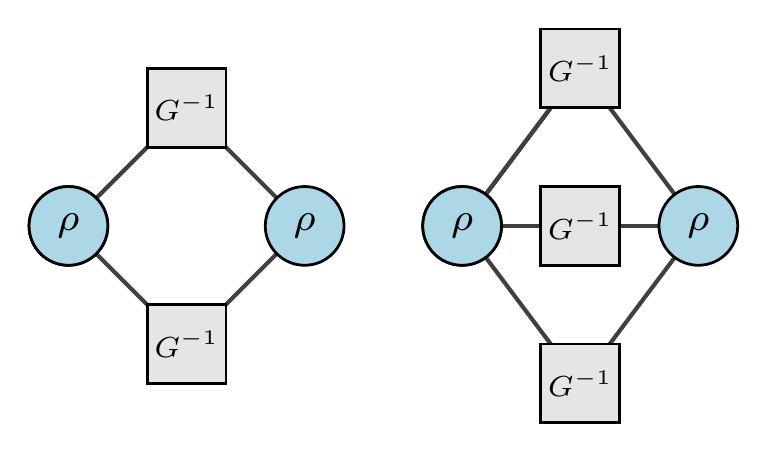
\begin{tikzpicture}
  \Vertex[size=1, label=$\rho$, fontscale=2]{A};
  \Vertex[x=1.5, y=1.5, size=1, shape=rectangle, color=gray!20, label=$G^{-1}$, fontscale=1.5]{B};
  \Vertex[size=1, label=$\rho$, fontscale=2]{A};
  \Vertex[x=3, y=0, size=1, label=$\rho$, fontscale=2]{C};
  \Vertex[x=1.5, y=-1.5, size=1, shape=rectangle, color=gray!20, label=$G^{-1}$, fontscale=1.5]{D};
  \Edge(A)(B);
   \Edge(B)(C);
    \Edge(C)(D);
     \Edge(D)(A);
     \begin{scope}[xshift= 5cm]
      \Vertex[size=1, label=$\rho$, fontscale=2]{A};
  \Vertex[x=1.5, y=2, size=1, shape=rectangle, color=gray!20, label=$G^{-1}$, fontscale=1.5]{B};
  \Vertex[size=1, label=$\rho$, fontscale=2]{A};
  \Vertex[x=3, y=0, size=1, label=$\rho$, fontscale=2]{C};
  \Vertex[x=1.5, y=-2, size=1, shape=rectangle, color=gray!20, label=$G^{-1}$, fontscale=1.5]{D};
  \Vertex[x=1.5, y=0, size=1, shape=rectangle, color=gray!20, label=$G^{-1}$, fontscale=1.5]{E};
  \Edge(A)(B);
  \Edge(A)(B);
   \Edge(B)(C);
    \Edge(C)(D);
     \Edge(D)(A);
     \Edge (A)(E);
     \Edge (E)(C);
     \end{scope}

 \end{tikzpicture}
\caption{On the left: Matrix product representation of the genus one conformal block in Eq.~\eqref{genus_one_conf_block}. On the right: Matrix product representation of the genus two conformal block in Eq.~\eqref{genus_two_conf_block}.}
\label{fig-g1}
\end{figure}

\subsection{Case $N=3$ (genus two)}\label{sec:genus_two}

For $N=3$, the orbifold three-point correlation 
function of Eq.~\eqref{N-point} can be computed 
by considering the three-to-one map~\cite{Collier}
\begin{equation}\label{g_two_covering_map}
 z(t) =\frac{(t+\omega)^3}{3\omega(1-\omega)t(t-1)},\quad \omega=e^{\frac{2\pi i}{3}}.
\end{equation}
This transformation has branch points of order three at 
$z=0$ and $1$ and maps the points $t_{\infty}=\{0, 1, \infty\}$ in the $t$-surface into $z=\infty$. 
Then we have that the orbifold three-point function in Eq.~\eqref{N-point} is in this case the three-point 
function of $\mathcal{C}$ on the sphere
\begin{align}\label{C_3_X}
 \langle \boldsymbol{\phi}^{\{M_1,M_2,M_3\}}_{\{h_1,h_2,h_3\}}(\infty) \sigma_{N}(1)\bar{\sigma}_{N}(0)\rangle &=\langle \tilde{\phi}_{h_1}^{M_1} (\infty) \tilde{\phi}_{h_2}^{M_2}(1) \tilde{\phi}_{h_3}^{M_3}(0)\rangle,
 = \\
 &=[3\omega(1-\omega)]^{-h_1-h_2-h_3}C_{h_1h_2h_3}\rho_{M1,M2,M3}^{h_1,h_2,h_3}
\end{align}
where $C_{h_1 h_2 h_3}=\langle \phi_{h_1}(\infty)\phi_{h_2}(1)\phi_{h_3}(0)\rangle$ is a structure constant in the seed CFT, while the symmetric tensor $\rho^{h_1,h_2,h_3}$ is 
\begin{equation}
\label{rho2}
 \rho^{h_1,h_2,h_3}_{M_1,M_2,M_3}:=
 \frac{\langle \mathcal{L}_{-M_1}\phi_{h_1}|\mathcal{L}_{-M_2}(1)\phi_{h_2}(1)|\mathcal{L}_{-M_3}\phi_{h_3}\rangle}
 { \langle \phi_{h_1}|\phi_{h_2}(1)|\phi_{h_3}\rangle}.
\end{equation}
The images $\mathcal{L}_{-n}(t_{\infty})$ of the Virasoro descendent $L_{-n}(z=\infty)$ 
under the conformal map in Eq.~\eqref{g_two_covering_map} can be obtained, as in the 
case $N=2$, by using Eq.~\eqref{Virasoro_transf}, see also Eq.~\eqref{vir_g2}.
The elements of Eq.~\eqref{rho2} can be calculated by implementing in a computer algebra system 
the Ward identities of Appendix~\ref{app_ward}. 
From Eq.~\eqref{C_3_X}, it follows that the $N=3$ orbifold conformal blocks are in one-to-one correspondence~\cite{Cardy, Collier} 
with the non-zero structure constants of $\mathcal{C}$.
After applying the map of Eq.~\eqref{g_two_covering_map} in Eq.~\eqref{conformal_block_decomposition},
we eventually obtain the following matrix-product representation for the $N=3$ orbifold conformal block \cite{Collier}
\begin{equation}\label{genus_two_conf_block}
 \mathcal{G}_{c, \{h_1, h_2, h_3\}}^{(3)}(z)=
z^{\sum_{j=1}^3 h_j-\frac{2c}{9}}\sum_{\substack{\{M_j\}, \{N_j\}}}
 z^{\sum\limits_{j=1}^3 |M_j|}
 \prod_{j=1}^3 [G_{M_j,N_j}^{h_j}]^{-1}
 \rho^{h_1,h_2,h_3}_{M_1,M_2,M_3}\rho_{N_3,N_2,N_1}^{h_3,h_2,h_1},
\end{equation}
which is also illustrated in Fig.~\ref{fig-g1}.
The conformal block $\mathcal{G}_{c, \{h_1, h_2, h_3\}}^{(3)}$ in Eq.~\eqref{genus_two_conf_block} is
manifestly symmetric under permutations of $h_1$, $h_2$ and $h_3$, consistently with the $\mathbb Z_3$ (in fact $S_3$) symmetry of the untwisted orbifold sector.

\subsection{Handling null vectors in minimal models}
\label{null_vec1}
We consider now the case in which the seed theory $\mathcal{C}$ has representations with {\it vanishing} null vector states \cite{BPZ}. 
In the following, we will focus on an important example of such theories, the minimal models $\mathcal{M}_{p,q}$, that have central charge
\begin{equation}
c=c_{p,q}= 1 -6\frac{ (p-q)^2}{p q},
\end{equation}
where $p$ and $q$ are integer coprimes. The minimal models are rational CFTs, i.e. they are built on a finite set of representations $\phi_{h^{p,q}_{r,s}}$ that is closed under OPE and with conformal dimensions
 \begin{equation}
 h^{p,q}_{r,s}=\frac{(q + p (-1 + r) - q s) (p (1 + r) - q (1 + s)}{4 p q}, \quad 1\leq r\leq q-1,  1\leq s\leq p-1.
 \end{equation}
Due to the chain of resonances $h_{r,s}^{p, q}=h_{q-r,p-s}^{p, q}=h_{q+r,p+s}^{p, q}=\cdots$, the representation $\phi_{h^{p,q}_{r,s}}$ has an infinite series of null vectors at the levels $r s, (q-r)(p-s),(q+r)(p+s), \dots$. Therefore, in order to compute the small $z$ expansion of the orbifold conformal blocks in the minimal models, $\mathcal{G}_{c_{p,q}, \boldsymbol{h}^{\text{deg}}}^{(N)}(z)$ with $\boldsymbol{h}^{\text{deg}}=\{h_{r_j, s_j}^{p, q}\}_{j=1}^N$, one has to choose a basis of descendents for each representation $h_{r_j, s_j}^{p, q}$ in which the null vectors have been removed. Even if there are closed expressions for the null vectors, it is quite complicated to implement this method, in particular considering the resonances mentioned above. We refer the reader to Ref.~\cite{Javerzat} where this particular issue is discussed in more detail. Here we will take an alternative strategy to deal with null vectors.
 
The sum in the small $z$ expansion of Eq.~\eqref{conformal_block_decomposition} runs over the standard basis of irreducible Verma modules; this sum  is not defined for minimal models. To see this, consider $\mathcal{G}_{c, \boldsymbol{h}^{\text{deg}}}^{(N)}(z)$, as given in Eq.~\eqref{conformal_block_decomposition}, as a function of $c$, $c\neq c_{p,q}$.  This conformal block presents then $0/0$ type singularities when $c=c_{p, q}$ at the levels where a null vector appears in one or more of the representations $h_{r_j, s_j}^{p, q}$. We propose here a simple regularization scheme of these singularities for $N=2$ and $3$ that allows to use the expansion of Eq.~\eqref{conformal_block_decomposition} and assures that the contribution of the null vectors and its descendants vanishes. This regularization procedure is in the same spirit as the one used for instance to apply the AGT relation to the minimal models.

The analytic properties of $\mathcal{G}_{c, \boldsymbol{h}^{\text{deg}}}^{(N)}(z)$ for $N=2$ and $3$ as a function of $c$ can be better understood by looking at the unfolded expressions of Eqs.~\eqref{C_2_X}~and~\eqref{C_3_X} respectively. At the level where there is a null vector in the representation $h_{r_j, s_j}^{p, q}$, the scalar product matrix $\left[G^{h^{p,q}_{r_j,s_j}}\right]^{-1}$ gives rise to a simple pole $(c-c_{p, q})^{-1}$, originated by the fact that the null vector is orthogonal to all the states.  At the same time, a simple zero $(c-c_{p,q})$ is produced by each $\rho$ term. For $N=2$, the latter is related to the cancellation of the scalar products $\rho^{h_{r,s}}$ between the null vector and any other basis state, see Eq.~\eqref{rho}, while, for $N= 3$, the vanishing of $\rho^{h_{r_1,s_1},h_{r_2,s_2},h_{r_3,s_3}}$ is connected with the fusion rules of the minimal model, see Eq.~\eqref{rho2}.  

Therefore, in order to eliminate the null vector contribution from Eqs.~\eqref{genus_one_conf_block} and \eqref{genus_two_conf_block}, 
it is enough, if $\boldsymbol{h}\neq \boldsymbol{0}$, to regularize the central charge differently in the $\rho$ and $G$ terms, 
that is to modify the central charge dependence of both $\rho^{\boldsymbol{h}^{\text{deg}}}$ and $G^{h_{r_j, p_j}^{p, q}}$ as follows
\begin{equation}\label{regularization}
 \rho^{\boldsymbol{h}^{\text{deg}}}|_{c_{p,q}+\varepsilon^2},\quad  G^{h_{r_j, s_j}^{p, q}}|_{c_{p,q}+\varepsilon},
\end{equation}
with $\varepsilon>0$. In this way, the singularities associated to the null vectors are always regularized and vanish 
in the limit $\varepsilon\to 0$, see also~\cite{SV, Alkalaev}. 

The case $\boldsymbol{h}=\boldsymbol{0}$ is a little bit different since the identity representation,
$h=0$, contains a null vector at level one for any value of the central charge. Hence we can follow 
a similar strategy but modifying the dependence of the matrices $G^{h}$ and $\rho^{\boldsymbol{h}}$
on $h$ and $\boldsymbol{h}$ instead of $c$ such that
\begin{equation}\label{regularization_identity}
 \rho^{\boldsymbol{h}=\{\mu^2,\dots, \mu^2\}}, G^{h=\mu},
\end{equation}
with $\mu>0$. Then the limit $\mu\to 0$ produces the regularized conformal block 
$\mathcal{G}_{c, \boldsymbol{0}}^{(N)}(z)$ for $N=2,3$. In particular, it provides, 
for $N=2$ and using Eq.~\eqref{character_conf_block}, the  character of the irreducible 
representation of the identity.

In the case $N=3$, note that, if the identity representation appears in only one of the copies, 
e.g. $h_1=0$, then, according to Eq.~\eqref{C_3_X},  we have to consider the same conformal family in the 
other two copies, i.e. $h_2=h_3$.  In order to obtain the correct conformal block in this situation,
one must take first $h_2=h_3$, with $h_1\neq 0$, and then perform the limit $h_1\to 0$. 

Let us see how regularization procedure presented above works in a particular example, the Ising field 
theory, which corresponds to take $p=5$ and $q=4$, and $c_{5, 4}=1/2$. For instance, for $h_{1, 2}=1/16$, 
the first few terms of the regularized expansion of Eq.~\eqref{genus_two_conf_block} about $z=0$ are 
\begin{equation}
 \mathcal{G}_{\frac{1}{2}, \frac{1}{16}}^{(2)}(z)=z^{1/8}
 \left[1+\frac{z}{16}+\frac{17z^2}{512}+\frac{187z^3}{8192}+\frac{9163z^4}{524288}+O(z^5)\right].
\end{equation}
The coefficient of the $O(z^4)$ term will be different if the regularization scheme is not implemented.
Indeed the representation $(c=1/2, h=1/16$) has a null vector at level two. If this vector was selected on both
replicas of the seed theory, i.e. in the sector $|M_1|=|M_2|=2$ of Eq.~\eqref{genus_one_conf_block}, it 
would give a non-zero contribution to the coefficient of the $O(z^4)$ term in the conformal block. 
If we take the regularization of Eq.~\eqref{regularization}, this contribution is of order $O(\varepsilon^2)$
and, therefore, drops in the limit $\varepsilon\to 0$.

As a second example, let us analyze the regularized $N=3$ orbifold conformal block for $c=1/2$ and $h_1=h_2=1/16$
and $h_3=0$; the result is 
\begin{equation}
 \mathcal{G}_{\frac{1}{2}, \{\frac{1}{16}, \frac{1}{16}, 0\}}^{(3)}(z)=
 z^{1/72}\left[1+\frac{7}{108}z^+\frac{1595}{46656}z^2+
 \frac{118405}{5038848}z^3+\frac{26160455}{1451188224}z^4+O(z^5)\right].
\end{equation}
Again, when the null vector at the second level 
of the representation $(c=1/2, h=1/16)$ appears in the sum of Eq.~\eqref{genus_two_conf_block} 
simultaneously in the two copies of $\mathcal{C}$ with this representation, 
it contributes to the $O(z^4)$ term. This spurious contribution is of order $O(\varepsilon^2)$ 
once we apply the regularization of Eq.~\eqref{regularization} and it is then removed in the
limit $\varepsilon\to0$.


\section{Orbifold conformal blocks in terms of sphere conformal blocks}\label{sec:sphere_conf_blocks}
Eq.~\eqref{conformal_block_decomposition} provides a small $|z|$ expansion of the modular conformal block of the type
\begin{equation}
\mathcal{G}_{c,\boldsymbol{h}}^{(N)}(z) =z^{|\boldsymbol{h}|-2h_{\sigma_N}} \;\sum_{j=0}^{\infty} a_j \; z^j.
\end{equation}
However, the computation of the coefficients $a_j$ becomes quickly impossible to accomplish and one has to approximate $\mathcal{G}_{c,\boldsymbol{h}}^{(N)}(z)$ by truncating the previous series at some value $L$,
\begin{equation}\label{trunc}
\mathcal{G}_{c,\boldsymbol{h}}^{(N)}(z) \sim z^{|\boldsymbol{h}|-2h_{\sigma_N}} \;\sum_{j=0}^{L} a_j \; z^j.
\end{equation}
In the case $N=3$, for instance, we are able to reach $L=6$.

A crucial point here is that the convergence of the series in Eq.~\eqref{conformal_block_decomposition} is slow close to  $|z|=1$. This, in turn, implies that, if the conformal block $\mathcal{G}_{c,\boldsymbol{h}}^{(N)}(z)$ is approximated by the truncated sum of Eq.~\eqref{trunc}, one misses the global properties of the twist field four-point function and, in particular, the crossing symmetry of Eq.~\eqref{cross_symmetry}. 
In Ref.~\cite{Collier}, this problem was tackled for $N=3$ by using a transformation from the frame $\Sigma_2(x)$ to the pillow frame. They  obtained then a series expansion in terms of the elliptic nome $q(z)=e^{i\pi\tau(z)}$, with $\tau(z)$ defined in Eq.~\eqref{tau}, 
of the form
\begin{equation}\label{collierap}
\mathcal{G}_{c,\boldsymbol{h}}^{(N)}(z) \sim z^{|\boldsymbol{h}|-2h_{\sigma_N}} \;\sum_{j=0}^{L} b_j \; q(z)^j.
\end{equation}
This expansion drastically improves the convergence properties of the twist field correlation function near $|z|=1$.

In this section, we will show how to improve the expansion of Ref.~\cite{Collier} by using a similar but different procedure.
As we discuss in detail in Appendix~\ref{app_orbifold_algebra}, the orbifold algebra admits as a sub-algebra a Virasoro algebra with central charge $Nc$~\cite{Borisov}, generated by the symmetric stress energy tensor in Eq.~\eqref{hatT}. Then it is natural to expand the orbifold conformal blocks 
$\mathcal{G}_{c, \boldsymbol{h}}^{(N)}(z)$ as a linear combination of Virasoro sphere conformal blocks with central charge $Nc$. More specifically,
\begin{equation}\label{expansion_sphere_conf_blocks}
 \mathcal{G}_{c, \boldsymbol{h}}^{(N)}(z)=\sum_{l=0}^\infty\alpha_l^{\boldsymbol{h}}\mathcal{F}_{Nc, |\boldsymbol{h}+l}(z),
\end{equation}
where we have  denoted by $\mathcal{F}_{Nc, h }(z)$ the Virasoro sphere conformal blocks with the four external dimensions fixed to  $h_{\sigma_N}$ and with internal channel of dimension $h$. The conformal block $\mathcal{F}_{Nc, |\boldsymbol{h}|+l}(z)$ resums the 
contribution of the conformal family generated by a field with conformal dimension $|\boldsymbol{h}|+l$, primary with respect to the 
orbifold Virasoro sub-algebra of Eq.~\eqref{symm_virasoro_alg}. The coefficients $\alpha_l^{\boldsymbol{h}}$ can be thought as Clebsch-Gordan coefficients for a 
decomposition of a $N$-fold tensor product of Virasoro algebra representations into a direct sum of irreducible representations with central charge $Nc$. A more detailed discussion concerning the meaning of Eq.~\eqref{expansion_sphere_conf_blocks}  as well as the algebraic nature of the coefficients $\alpha_{l}^{\boldsymbol{h}}$ can be found in subsection~\ref{deralpha}. The fine structure of the orbifold algebra was used in Ref.~\cite{Dupic} to derive differential equations for certain twist field correlation functions.

Now observe that, if we truncate Eq.~\eqref{expansion_sphere_conf_blocks}  
\begin{equation}\label{expansion_sphere_conf_blocks_trunc}
 \mathcal{G}_{c, \boldsymbol{h}}^{(N)}(z)\sim\sum_{l=0}^{L}\alpha_{l}^{\boldsymbol{h}}
 \mathcal{F}_{Nc, |\boldsymbol{h}|+l}(z),
\end{equation}
then the coefficients $\alpha_{l}^{\boldsymbol{h}}$ can be easily derived by expanding $\mathcal{F}_{Nc, |\boldsymbol{h}|+l}(z)$ in power series and identifying order by order the sums of Eqs.~\eqref{trunc} and \eqref{expansion_sphere_conf_blocks_trunc}.
Eq.~\eqref{expansion_sphere_conf_blocks_trunc} is already a better approximation than 
Eq.~\eqref{trunc}, as each  $\mathcal{F}_{Nc, |\boldsymbol{h}|+l}(z)$ can be computed until orders much bigger than $z^{|\boldsymbol{h}|-2h_{\sigma_N}+L}$. In other words, this means that we can take into account the contribution of certain very low descendants of the orbifold algebra that were previously unaccessible.


The second step is to express the $\mathcal{F}_{N c, |h }(z)$ as an expansion in terms of the elliptic nome $q(z)$ by using the elliptic Zamolodchikov recursion relation~\cite{Zamolodchikov2},
\begin{equation}\label{zam_recursion}
 \mathcal{F}_{Nc, h}(z)=
 f_N(q(z), c, h) \;H(Nc, h, h_{\sigma_N}, q(z)),
\end{equation}
where
\begin{align}
f_N(q, c, h) &= 16^{\frac{1-Nc}{24}}q(z)^{h-\frac{Nc-1}{24}}
 [z(1-z)]^{\frac{Nc-1}{24}-2h_{\sigma_N}}
 \vartheta_3(q(z))^{\frac{Nc-1}{2}-16h_{\sigma_N}}, \\
 H_N(q, c, h)&=1+\sum_{j=1}^{\infty}d_j(c, h,N)\;q^j.
\end{align}
The coefficients $d_j(c, h,N) $ can be computed recursively to very large values of $j$, see Ref.~\cite{Zamolodchikov2}. 

Finally, combining Eqs.~\eqref{expansion_sphere_conf_blocks_trunc} and \eqref{zam_recursion}, we obtain the following approximation 
for $\mathcal{G}_{c, \boldsymbol{h}}^{(N)}(z)$, 
\begin{equation}
\label{usap}
\mathcal{G}_{c,\boldsymbol{h}}^{(N)}(z) \sim z^{|\boldsymbol{h}|-2h_{\sigma_N}} \left(\sum_{j=0}^{L} b_j \; q(z)^j+\sum_{j=L+1}^{L'} c_j q(z)^{j}\right), 
\end{equation}
that provides sub-leading corrections to Eq.~\eqref{collierap}. It is important to stress that both Eqs.~\eqref{collierap}~and~\eqref{usap} approximate the conformal block $ \mathcal{G}_{c,\boldsymbol{h}}^{(N)}(z)$ with an error $o(q(z)^{L})$. However, the $q^j$ terms with $j>L$  in Eq.~\eqref{usap} come from the contribution of (some of) the descendent fields at level $j$, thus it gives a better approximation than Eq.~\eqref{collierap}.  

\subsection{Orbifold algebra and algebraic nature of the $\alpha_{l}^{{\bf h}}$}\label{deralpha}

To illustrate the main idea behind Eq.~\eqref{expansion_sphere_conf_blocks}, it is sufficient to consider the first level contribution to  
$\mathcal{G}_{c, \boldsymbol{h}}^{(N)}(z)$ for the case $N=3$. If we explictly calculate the first order term in the expansion of Eq.~\eqref{genus_two_conf_block}, we have that
\begin{equation}
\mathcal{G}_{c, \boldsymbol{h}}^{(3)}(z)= z^{|\boldsymbol{h}|-2h_{\sigma_N}}\left[1+\left(\frac{|\boldsymbol{h}|}{2}+\frac{1}{54}\left(\frac{(h_1-h_2)^2}{h_3}+\frac{(h_1-h_3)^2}{h_2}+\frac{(h_2-h_3)^2}{h_1}\right)\right)\;z+O(z^2)\right],
\end{equation}
where we recall that here $\boldsymbol{h}=\{h_1,h_2,h_3\}$ and $|\boldsymbol{h}|=h_1+h_2+h_3$. The conformal block $\mathcal{G}_{c, \boldsymbol{h}}^{(3)}(z)$ is associated with the field $\boldsymbol{\phi}_{\boldsymbol{h}}=\phi_{h_1}\otimes\phi_{h_2}\otimes\phi_{h_3}$ and its descendents. In particular, the coefficient of the $z^{|\boldsymbol{h}|-2h_{\sigma_N}+1}$ term comes from the contribution of three descendants,
\begin{equation}
|v_1\rangle =L_{-1}\phi_{h_1}\otimes \phi_{h_2}\otimes \phi_{h_3},   \quad |v_2\rangle =\phi_{h_1}\otimes  L_{-1}\phi_{h_2}\otimes \phi_{h_3},\quad |v_3\rangle=\phi_{h_1}\otimes \phi_{h_2}\otimes  L_{-1} \phi_{h_3}.
\end{equation}

The symmetric linear combination of the three states above corresponds to the descendant of the orbifold Virasoro sub-algebra
of Eq.~\eqref{symm_virasoro_alg}
\begin{equation}
\boldsymbol{L}_{-1}\boldsymbol{\phi}_{\boldsymbol{h}}=|v_1\rangle+|v_2\rangle+|v_3\rangle.
\end{equation} 
This descendant contributes with the term with coefficient $|\boldsymbol{h}|/2$ to the expansion of Eq.~\eqref{usap}. This contribution is taken into account by the first Virasoro sphere conformal block in the expansion of Eq.~\eqref{expansion_sphere_conf_blocks}. In fact, 
\begin{equation}
\mathcal{F}_{3c, |\boldsymbol{h}|}(z)=z^{|\boldsymbol{h}|-2h_{\sigma_N}}\left[1+\frac{|\boldsymbol{h}|}{2}z+O(z^2)\right].
\end{equation}

Let us take now the space of states that are orthogonal to $\boldsymbol{L}_{-1}\boldsymbol{\phi}_{\boldsymbol{h}}$. This is a two dimensional space of states $|v\rangle_{\lambda}$ parametrized by $\lambda \in \mathbb{C}$ of the form
\begin{equation}
\label{ortosub}
 |v\rangle_{\lambda}= |v_1\rangle+\lambda |v_2\rangle
 -\frac{h_1+\lambda h_2}{h_3} |v_3\rangle.
\end{equation}
One can check
that any vector in this orthogonal space is a primary of the $3 c$ Virasoro sub-algebra of 
Eq.~\eqref{symm_virasoro_alg}, i.e. $\boldsymbol{L}_n  |v\rangle_{\lambda}=0$ for all $n>0$
and $\boldsymbol{L}_0|v\rangle_{\lambda} = (h_1+h_2+h_3+1)|v\rangle_{\lambda}$.
The contribution of these states and their symmetric descendents $\boldsymbol{L}_{-M}|v\rangle_{\lambda}$ 
to the conformal block $\mathcal{G}_{c, \boldsymbol{h}}^{(3)}(z)$ is given by
\begin{equation}
\alpha_{1}^{\boldsymbol{h}}\;\mathcal{F}_{3c, |\boldsymbol{h}|+1}(z),
\end{equation}
where 
\begin{equation}
\label{alpha1}
\alpha_{1}^{\boldsymbol{h}} =\frac{1}{54}\left[\frac{(h_1-h_2)^2}{h_3}+\frac{(h_1-h_3)^2}{h_2}+\frac{(h_2-h_3)^2}{h_1}\right].
\end{equation}
The coefficient $\alpha_{1}^{\boldsymbol{h}}$ can  be determined by choosing two particular values of $\lambda$, say $\lambda_1$ and $\lambda_2$, such that $\{|v\rangle_{\lambda_1}, |v\rangle_{\lambda_2}\}$ is an orthonormal basis of the orthogonal subspace of Eq.~\eqref{ortosub}. Then one can obtain the result of Eq.\eqref{alpha1} from the expression
\begin{eqnarray}
 \alpha_1^{\boldsymbol{h}}&=&\frac{1}{D_{\boldsymbol{h},\boldsymbol{\bar{h}}}}\left[(_{\lambda_1}\langle v |\otimes \langle \boldsymbol{\phi}_{\boldsymbol{\bar{h}}}|)\sigma_{3}(1)|\bar{\sigma}_3\rangle \;\langle \sigma_{3}|\bar{\sigma}_3(1) (|v\rangle_{\lambda_1}\otimes |\boldsymbol{\phi}_{\boldsymbol{\bar{h}}}\rangle)  \right.+\\ 
 &+&\left.
 ( _{\lambda_2}\langle v| \otimes \langle \boldsymbol{\phi}_{\boldsymbol{\bar{h}}}|)|\sigma_{3}(1)|\bar{\sigma}_3\rangle \;\langle \sigma_{3}|\bar{\sigma}_3(1)(|v\rangle_{\lambda_2}\otimes |\boldsymbol{\phi}_{\boldsymbol{\bar{h}}}\rangle)  \right]
\end{eqnarray}
where $D_{\boldsymbol{h},\boldsymbol{\bar{h}}}$ is related to the structure constant as in Eq.~\eqref{DC}. As we already pointed out for the matrix elements $\Gamma$ and $\Gamma^*$, defined in Eq.~\eqref{Gammas}, the coefficient $\alpha^{\boldsymbol{h}}_1$  is algebraic in nature, despite the holomorphic and anti-holomorphic fields appear in the equation above. This can be seen from the fact they are rational functions of the central charge $c$ and of the holomorphic dimensions $h_j$.

The states $\boldsymbol{L}_{-M}\boldsymbol{\phi}_{\boldsymbol{h}}$ and $\boldsymbol{L}_{-M} |v\rangle_{\lambda}$ 
do not span the full space of descendents of $\boldsymbol{\phi}_{\boldsymbol{h}}$ for levels greater than one. 
This is the reason why other Virasoro conformal blocks appear and one finally gets the expansion of Eq.~\eqref{expansion_sphere_conf_blocks}. 
In fact, the previous analysis may be extended to deeper levels and generalized to any number of copies $N$.
If we denote by $\mathfrak{p}(l)$ the number of partitions of the integer $l$, then there are $\mathfrak{p}(l)$ symmetric
descendents $\boldsymbol{L}_{-M}\boldsymbol{\phi}_{\boldsymbol{h}}$ at level $l$. However,
for an arbitrary number of copies $N$ and assumming that there are no null vectors, it is easy to check that 
at level $l$ the total number $\mathcal{N}_{N, l}$ of linear independent descendents of $\boldsymbol{\phi}_{\boldsymbol{h}}$ is
\begin{equation}
 \mathcal{N}_{N, l}=\sum_{\substack{Y, |Y|=l \\ |j_Y|\leq N}}\frac{N!}{(N-|j_Y|)!
 \prod_{i=1}^{|i_Y|}d_Y(i)!}\prod_{j=1}^{|j_Y|}\mathfrak{p}(i_Y(j)),
\end{equation}
where $Y$ denotes a partition of $l$. If we consider the Young tableau
associated to $Y$, then $|i_Y|$ and  $|j_Y|$ denote its number of columns and
rows respectively, $i_Y(j)$ is the number of columns in the row $j$ and 
$d_Y(i)$ is the number of rows with $i$ columns.

Therefore, at level $l$, we will find a set of $\tilde{\mathcal{N}}_{N,l}$ orthonormal fields 
$|v\rangle_j$, $j=1,\dots, \tilde{\mathcal{N}}_{N,l}$,
such that $\boldsymbol{L}_0 |v\rangle_j=(|\boldsymbol{h}|+l)|v\rangle_j$ and are primaries,
$\boldsymbol{L}_n|v\rangle_j=0$ for all $n>0$. These primaries have associated the 
sphere conformal block $\mathcal{F}_{Nc, |\boldsymbol{h}|+l}(z)$, which gives the 
contribution of these vectors and their symmetric descendents $\boldsymbol{L}_{-M}|v\rangle_j$
to the orbifold conformal block $\mathcal{G}_{c, \boldsymbol{h}}^{(N)}(z)$, 
according to Eq.~\eqref{expansion_sphere_conf_blocks}. The corresponding structure constant $\alpha_l^{\boldsymbol{h}}$
is given by
\begin{equation}\label{alpha_l}
 \alpha_l^{\boldsymbol{h}}=\frac{1}{D_{\boldsymbol{h},\boldsymbol{\bar{h}}}}\sum_{j=1}^{\tilde{\mathcal{N}}_{N,l}}
 (_{\lambda_j}\langle v |\otimes \langle \boldsymbol{\phi}_{\boldsymbol{\bar{h}}}|)\sigma_{3}(1)|\bar{\sigma}_3\rangle \;\langle \sigma_{3}|\bar{\sigma}_3(1) (|v\rangle_{\lambda_j}\otimes |\boldsymbol{\phi}_{\boldsymbol{\bar{h}}}\rangle).
\end{equation}
The primary fields at 
different levels, as well as their descendents, are orthogonal
since they belong to different representations of the Virasoro algebra of Eq.~\eqref{symm_virasoro_alg}.
%If there are no null vectors, then the number of primaries at level $l$ is
%\begin{equation}
% \tilde{\mathcal{N}}_{N, l}=\mathcal{N}_{N, l}
% -\sum_{m=0}^{l-1}\tilde{\mathcal{N}}_{N, m}\mathfrak{p}(l-m).
%\end{equation}
\section{Applications}\label{sec:num_bootstrap}

\subsection{Entanglement of disjoint intervals}

A first application of the results of the previous sections is in 
the analysis of the spatial entanglement in the ground state of a 
unidimensional quantum model at a critical point. Let us suppose that 
the system can be divided into two spatial regions $A$ and $B$. The entanglement
between these two subsystems can be characterized by the moments $\Tr\rho_A^N$
of the reduced density matrix $\rho_A$, defined in Eq.~\eqref{red_density_matrix} 
of Appendix~\ref{app_ent}. We will further consider that subsystem $A$ consists 
of two disjoint regions $A_1$ and $A_2$, i.e. $A=A_1\cup A_2$. Then one can also 
study the entanglement between $A_1$ and $A_2$, which can be quantified by the moments 
$\Tr (\rho_A^{T_2})^N$ of the partial transpose of $\rho_A$, which we will denote by $\rho_A^{T_2}$
and defined in Eq.~\eqref{partial_transpose}.

Now we suppose that the universal properties of the quantum model at the critical 
point are determined by the CFT $\mathcal{C}$. Without loss of generality, we can 
take as regions $A_1$ and $A_2$ the intervals $A_1=(0, x)$ and $A_2=(1, \infty)$, 
with $0<x<1$. Then the moments $\Tr \rho_A^N $ and $\Tr (\rho_A^{T_2})^N$ are equal to 
 \begin{equation}\label{red_mat_ft}
 \Tr\rho_A^N=K_N\langle \sigma_N(0)\bar{\sigma}_N(x)\sigma_N(1)\bar{\sigma}_N(\infty)\rangle,
 \end{equation}
 and
 \begin{equation}\label{partial_trans_ft}
 \Tr(\rho_A^{T_2})^N=K_N\langle \sigma_N(0)\bar{\sigma}_N(x)\bar{\sigma}_N(1)\sigma_N(\infty)\rangle,
 \end{equation}
where $K_N$ is a non universal constant. Note that the partial transposition crucially exchanges the twist and anti-twist operators 
at the points $z=1$ and $\infty$. The crossing transformation $z\mapsto 1-z$ maps subsystem 
$A=(0, x)\cup(1, \infty)$ into its complement $B=(-\infty, 0)\cup(1-x, 1)$. Thus
the crossing invariance of the four point correlation function $\langle \sigma_N(0)
\bar{\sigma}_N(x) \sigma_N(1) \bar{\sigma}_N(\infty)\rangle$ implies that $\Tr\rho_A^N=\Tr\rho_B^N$
and, therefore, the well-known property that for a pure state the entanglement entropies of a 
subsystem and its complementary are equal. This is not true for the moments $\Tr(\rho_A^{T_2})^N$
and, in fact, the four point function $ \langle \sigma_N(0)\bar{\sigma}_N(x)\bar{\sigma}_N(1)\sigma_N(\infty)\rangle$
is not crossing invariant. For the case $N=2$, since the twist and anti-twist fields are identical, $\sigma_2=\bar{\sigma}_2$, 
then $\Tr\rho_A^2=\Tr(\rho_A^{T_2})^2$. 

The correlation functions of Eqs.~\eqref{red_mat_ft} and \eqref{partial_trans_ft} are
related by the conformal transformation
\begin{equation}
 y(z)=\frac{z}{z-1},
\end{equation}
which maps the points $(0, x, 1, \infty)$ into $(0, x/(x-1), \infty, 1)$, such that
\begin{equation}
 \langle \sigma_N(0)\bar{\sigma}_N(x)\bar{\sigma}_N(1)\sigma_N(\infty)\rangle=
 (1-x)^{-4h_\sigma}\langle \sigma_N(0)\bar{\sigma}_N(x/(x-1))\sigma_N(1)\bar{\sigma}_N(\infty)\rangle,
\end{equation}
and we can rewrite Eq.~\eqref{partial_trans_ft} in the form 
\begin{equation}\label{partial_trans_ft_2}
 \Tr(\rho_A^{T_2})^N=K_N(1-x)^{-4h_\sigma}\langle \sigma_N(0)\bar{\sigma}_N(x/(x-1))\sigma_N(1)\bar{\sigma}_N(\infty)\rangle.
 \end{equation}
Thus, while for $\Tr\rho_A^N$ we need to calculate the correlation function 
$\langle\sigma_N(0)\bar{\sigma}_N(x)\sigma_N(1)\bar{\sigma}_N(\infty)\rangle$
in the interval $0<x<1$, the computation of $\Tr(\rho_A^{T_2})^N$ requires to consider it
for $x/(x-1)<0$. Therefore, in the case of the moments $\Tr\rho_A^N$, we can directly apply 
the results of the previous sections, in particular Eqs.~\eqref{conformal_block_decomposition_0}
and \eqref{expansion_sphere_conf_blocks}, and we have
\begin{equation}\label{red_mat_cb}
 \Tr\rho_A^N=K_N\sum_{\boldsymbol{h}, \boldsymbol{\bar{h}}}\sum_{l, l'} 
 \tilde{D}_{\boldsymbol{h}, \boldsymbol{\bar{h}}}^{l, l'} 
 \mathcal{F}_{Nc, |\boldsymbol{h}|+l}(x)\mathcal{F}_{Nc, |\boldsymbol{\bar{h}}|+l'}(x)
\end{equation}
with $\tilde{D}_{\boldsymbol{h}, \boldsymbol{\bar{h}}}^{l, l'}=D_{\boldsymbol{h}, 
\boldsymbol{\bar{h}}}\alpha_l^{\boldsymbol{h}}\alpha_{l'}^{\boldsymbol{\bar{h}}}.$
On the other hand, to obtain a similar result for $\Tr(\rho_A^{T_2})^N$, 
one must find the analytic continuation of the twist-field correlation function to 
the negative axis. This can be straightforwardly done from the expression of conformal 
blocks in terms of the elliptic nome $q(x)=e^{i\pi \tau(x)}$. In fact, note that
\begin{equation}\label{tau_p_1}
 \tau\left(\frac{x}{x-1}\right)=\tau(x)+1, \quad \text{and} \quad 
 q\left(\frac{x}{x-1}\right)=e^{i\pi} q(x).
\end{equation}
Hence $\Tr(\rho_A^{T_2})^N$ can also be expanded by using Eqs.~\eqref{conformal_block_decomposition_0} 
and \eqref{expansion_sphere_conf_blocks} but evaluating now
the Virasoro conformal blocks at $e^{i\pi}q(x)$,
\begin{equation}\label{partial_trans_cb}
 \Tr(\rho_A^{T_2})^N=K_N(1-x)^{-4h_\sigma}\sum_{\boldsymbol{h}, \boldsymbol{\bar{h}}}\sum_{l, l'} 
 \tilde{D}_{\boldsymbol{h}, \boldsymbol{\bar{h}}}^{l, l'} 
 \mathcal{F}_{Nc, |\boldsymbol{h}|+l}(e^{i\pi}q)\mathcal{F}_{Nc, |\boldsymbol{\bar{h}}|+l'}(e^{-i\pi}q).
\end{equation}
Note that, for convenience, we have changed here $x$ for the elliptic nome $q$ 
as the argument of $\mathcal{F}_{Nc, h}$, we will only maintain this notation in 
the following equations. Observe that, for $N=2$, Eq.~\eqref{tau_p_1} corresponds to perform the modular 
transformation $\tau(x)\mapsto \tau(x)+1$ on the modulus of the torus $\Sigma_1(x)$.
Then $\hat{\mathcal{Z}}_1(x)$ and $\hat{\mathcal{Z}}_1(x/(x-1))$ are the partition functions
of $\mathcal{C}$ on a flat torus of moduli $\tau(x)$ and $\tau(x)+1$ respectively. Taking into account Eqs.
\eqref{red_mat_ft} and \eqref{partial_trans_ft_2}, the invariance of the partition function on the torus under modular transformations, 
$\hat{\mathcal{Z}}_1(x)=\hat{\mathcal{Z}}_1(x/(x-1))$, leads to the identity $\Tr\rho_A^2=\Tr(\rho_A^{T_2})^2$ anticipated before.

We can cast Eq.~\eqref{partial_trans_cb} in a simpler and suggestive form. If we take the 
Zamolodchikov recursion for the Virasoro conformal blocks and we apply 
the following identities of the Jacobi theta functions
\begin{equation}
 \vartheta_2(e^{\pm i\pi}q)=e^{\pm i\pi/4}\vartheta_2(q), \quad 
 \vartheta_3(e^{\pm i\pi}q)=\vartheta_4(q), \quad 
 \vartheta_4(e^{\pm i\pi}q)=\vartheta_3(q),
\end{equation}
and 
\begin{equation}
 x=\left(\frac{\vartheta_2(q)}{\vartheta_3(q)}\right)^4, \quad 
 1-x=\left(\frac{\vartheta_4(q)}{\vartheta_3(q)}\right)^4,
\end{equation}
one can show that 
\begin{equation}
 \mathcal{F}_{Nc, h}(e^{\pm i\pi}q)=e^{\pm i\pi(h-2h_{\sigma_N})}
 (1-x)^{2h_{\sigma_N}}\mathcal{F}_{Nc, h}(q).
\end{equation}
Plugging this identity into Eq.~\eqref{partial_trans_cb}, the conformal block
expansion of the moments $\Tr(\rho_A^{T_2})^N$ can be rewritten
in the form
\begin{equation}\label{partial_trans_cb_2}
 \Tr(\rho_A^{T_2})^N=K_N\sum_{\boldsymbol{h}, \boldsymbol{\bar{h}}}\sum_{l, l'} 
 e^{i\pi(|\boldsymbol{h}|-|\boldsymbol{\bar{h}}|+l-l')}\tilde{D}_{\boldsymbol{h}, \boldsymbol{\bar{h}}}^{l, l'} 
 \mathcal{F}_{Nc, |\boldsymbol{h}|+l}(x)\mathcal{F}_{Nc, |\boldsymbol{\bar{h}}|+l'}(x).
\end{equation}  
If we compare this result with Eq.~\eqref{red_mat_cb}, the moments $\Tr(\rho_A^{T_2})^N$
have the same Virasoro conformal block decomposition as $\Tr(\rho_A^{T_2})^N$, 
but with the structure constants multiplied by a phase that depends on
the spin $|\boldsymbol{h}|-|\boldsymbol{\bar{h}}|+l-l'$ of the corresponding primary field. 
Then we conclude that
\begin{equation}
 \Tr\rho_A^N-\Tr(\rho_A^{T_2})^N=\text{sum over the channels with spin}\,\,
 |\boldsymbol{h}|-|\boldsymbol{\bar{h}}|+l-l'\neq 2k,\quad k\in\mathbb{Z}.
\end{equation}
Note that, in the case $N=2$, due 
to the identity $\Tr\rho_A^2=\Tr(\rho_A^{T_2})^2$, the channels indicated above cannot appear in the 
conformal block decompositions of $\Tr\rho_A^2$ and $\Tr(\rho_A^{T_2})^2$.


To the best of our knowledge, analytic expressions of $\Tr\rho_A^N$ and $\Tr(\rho_A^{T_2})^N$ have  
only been obtained for the compactified massless boson, the massless Dirac 
model and the Ising field theory. Here we shall consider the latter. In order 
to compare with the previous literature, let us write the moments $\Tr\rho_A^N$ 
and $\Tr(\rho_A^{T_2})^N$ in the form
\begin{equation}\label{F_n_cc}
\Tr\rho_A^N=K_Nx^{-4h_\sigma}(1-x)^{-4h_\sigma}\mathcal{R}_N(x)
\end{equation}
and 
\begin{equation}\label{G_n_cc}
 \Tr(\rho_A^{T_2})^N=K_N x^{-4h_\sigma}(1-x)^{4h_\sigma}\mathcal{R}_N\left(\frac{x}{x-1}\right).
\end{equation}
In Refs. xxx and xxx, an exact expression of the function
$\mathcal{R}_N(z)$, $z\in\mathbb{C}$, was obtained for the Ising field theory, 
which can be found in Eq.~\eqref{R_n_ising} of Appendix~\ref{app_ising}. 
We have checked that Eq.~\eqref{R_n_ising} is exactly reproduced in the intervals $0<x<1$ and $x/(x-1)<0$ by the 
conformal block expansions of Eqs.~\eqref{red_mat_cb} and \eqref{partial_trans_cb_2} 
respectively. In Appendix~\ref{app_ising}, we write the explicit 
conformal block decomposition, with the values of the structure constants, 
of the twist-field four-point function in the Ising model for $N=3$ up to sixth order. 

\begin{figure}[t]
 \begin{minipage}{0.5\linewidth}
 \centering 
 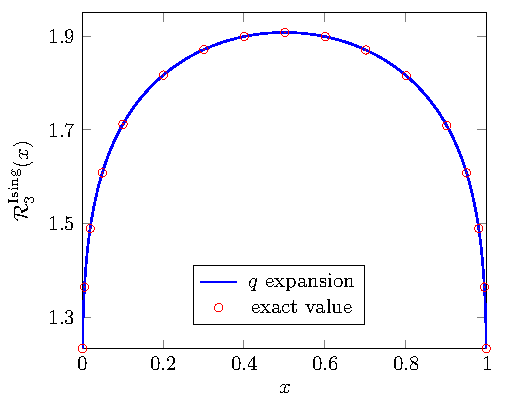
\includegraphics[width=\textwidth]{renyi_entropy_3_ising.pdf}
\end{minipage}
 \begin{minipage}{0.5\linewidth}
 \centering 
 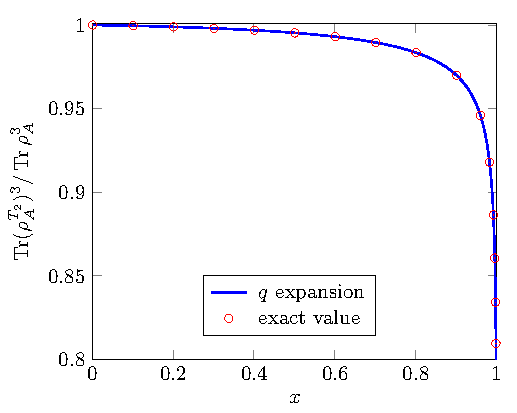
\includegraphics[width=\textwidth]{quotient_negativity_entropy_3_ising.pdf}
\end{minipage}
\caption{}\label{fig:ent_ising}
\end{figure}


In Fig.~\ref{fig:ent_ising} left, we plot the function $\mathcal{R}_3^{\text{Ising}}(x)$. 
The solid line has been drawn by employing the conformal block expansion of Eq.~\eqref{red_mat_cb} 
for $\Tr\rho_A^3$ and the dots are the exact values given by Eq.~\eqref{R_n_ising}. 
The agreement between both results is excellent. Note that, due to the crossing symmetry of the 
twist-field four-point function and, therefore, of $\Tr\rho_A^N$, $\mathcal{R}_N(x)$ must 
satisfy in general that $\mathcal{R}_N(x)=\mathcal{R}_N(1-x)$.
In Fig.~\ref{fig:ent_ising} right, we plot the quotient $\Tr(\rho_A^{T_2})^3/\Tr\rho_A^3$. 
The solid curve has been obtained using the conformal block expansions of Eq.~\eqref{red_mat_cb} 
and \eqref{partial_trans_cb_2} for $\Tr\rho_A^3$ and $\Tr(\rho_A^{T_2})^3$ while 
the dots have been calculated from the quotient of Eqs.~\eqref{F_n_cc} and \eqref{G_n_cc} 
and applying Eq.~\eqref{R_n_ising} for the function $\mathcal{R}_3$. Again the conformal block
expansion perfectly matches with the former known results.

\begin{figure}[t]
 \begin{minipage}{0.5\linewidth}
 \centering 
 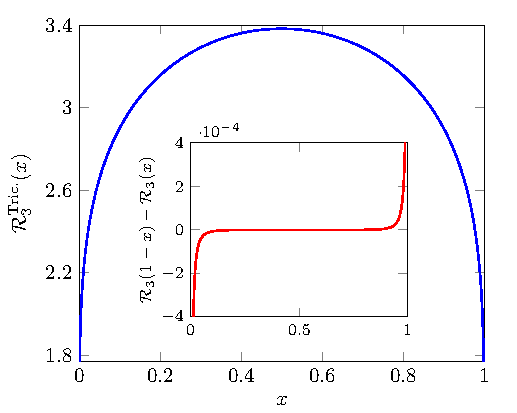
\includegraphics[width=\textwidth]{renyi_entropy_3_tricritical.pdf}
\end{minipage}
 \begin{minipage}{0.5\linewidth}
 \centering 
 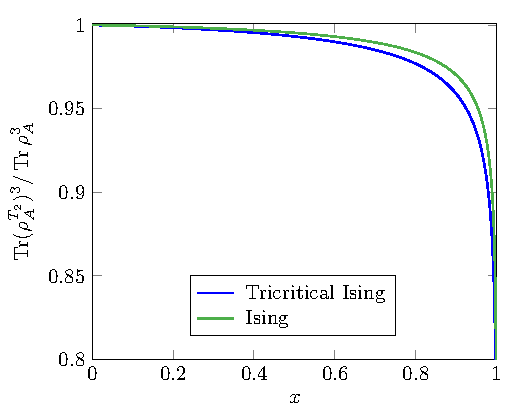
\includegraphics[width=\textwidth]{quotient_negativity_entropy_3_tricritical.pdf}
\end{minipage}
\caption{}\label{fig:ent_tricritical}
\end{figure}

In Fig.~\ref{fig:ent_tricritical}, we consider the moments $\Tr\rho_A^3$ and 
$\Tr(\rho_A^{T_2})^3$ for the Tricritical Ising model, for which there are not 
previous results in the literature. In Fig.~\ref{fig:ent_tricritical} left, we plot 
the function $\mathcal{R}_3(x)$ for this theory, obtained from the corresponding conformal block 
decomposition of $\Tr\rho_A^3$. In Appendix xxx, one can find the explict conformal block expansion, 
as well as the values of the structure constants, of the twist-field four-point function for the 
Tricrtical Ising model when $N=3$ up to sixth order. In the inset, we check the crossing-symmetry 
of $\mathcal{R}_3^{\text{Tric.}}(x)$ using the conformal block expansion. We obtain a very good 
symmetry when we change $x$ by $1-x$. In Fig.~\ref{fig:ent_tricritical} right, we plot the quotient 
of moments $\Tr(\rho_A^{T_2})^3/\Tr\rho_A^3$ using the conformal block decomposition of Eqs.~\eqref{red_mat_cb} and \eqref{partial_trans_cb_2}.  Here we also compare with the results found for the Ising model, the dashed line. 



\subsection{Constraints on the structure constants}

In Ref.~\cite{Collier}, the crossing symmetry of the twist field four-point 
function for the case $N=3$ was employed to extract some non trivial constraints on the 
structure constants of the seed theory $\mathcal{C}$. For this purpose, the authors mapped 
the orbifold conformal block $\mathcal{G}_{c, \boldsymbol{h}}^{(3)}(z)$ from the 
twist field frame to the 3-fold pillow frame, which makes apparent some positivity properties of 
the block for unitary theories. As we already mentioned in Sec.~\ref{sec:sphere_conf_blocks}, this transformation
produces a series for the orbifold conformal block in terms of the elliptic nome $q(z)$
of the form of Eq.~\eqref{collierap}. In this subsection, we will see how to rederive 
such constraints on the structure constants from the expansion of the orbifold 
conformal blocks in terms of the ones on the sphere, studied in Sec.~\ref{sec:sphere_conf_blocks}. This 
expansion results in a power series expansion in $q(z)$ of the form of Eq.~\eqref{usap}
Therefore, as we will see, it provides slightly tighter contraints on the structure
constants than the expansion used in Ref.~\cite{Collier}.

First, as in Ref.~\cite{Collier}, we must recast the Zamolodchikov recursion relation, Eq.~\eqref{zam_recursion}, 
for the Virasoro conformal blocks $\mathcal{F}_{Nc, h}(z)$ in order to make manifest 
certain positivity properties of it that we will need later. More specifically, the 
coefficients $d_j$ of the factor $H(Nc, h, h_{\sigma_N}, q)$ are not in general positive
definite. We can get it positive in unitary theories by reinterpreting the Zamolodchikov recursion
relation as in Ref.~\cite{Maldacena}. In that paper, the conformal block $\mathcal{F}_{Nc, h}(z)$, 
which is defined on the sphere, is mapped to the pillow (the quotient of a flat torus
by $\mathbb{Z}_2$, which is topologically equivalent to a sphere with four conical singularities). 
The important result for us is that the transformed blocks $\tilde{\mathcal{F}}_{Nc, h}(z)$ read 
\begin{equation}
 \tilde{\mathcal{F}}_{Nc, h}(q)=\mathcal{\vartheta}_3(q)^{16h_{\sigma_N}-\frac{Nc}{2}}
 \left[z(1-z)\right]^{2h_{\sigma_N}-\frac{Nc}{24}}\mathcal{F}_{Nc, h}(z),
\end{equation}
and, if $\tilde{\mathcal{F}}_{Nc, h}(z)$ is interpreted as a sum over the states on the pillow, 
then it admits the expansion
\begin{equation}
 \tilde{\mathcal{F}}_{Nc, h}(q)=q^{h-\frac{Nc}{24}}\sum_{l=0}^\infty \tilde{a}_n(h) q^{n},
\end{equation}
where the coefficients $\tilde{a}_n(h)$ are sums of scalar products between the descendent states at level $n$ 
and, consequently, they are non-negative, $\tilde{a}_n(h)\geq 0$, for unitary theories. Therefore, we 
can rewrite the Virasoro conformal blocks in the form
\begin{equation}\label{Vir_cb_pillow}
 \mathcal{F}_{Nc, h}(z)=q^{h-\frac{Nc}{24}}\left[z(1-z)\right]^{\frac{Nc}{24}-2h_{\sigma_N}}
 \vartheta_3(q)^{\frac{Nc}{2}-16h_{\sigma_N}}\sum_{n=0}^\infty \tilde{a}_n(h) q^n.
\end{equation}
The coefficients $\tilde{a}_n(h)$ can be easily computed from the Zamolodchikov recursion relation.

If we now truncate at order $L'>L$ the power series of Eq.~\eqref{Vir_cb_pillow} and insert it into the truncated
expansion of $\mathcal{G}_{c, \boldsymbol{h}}(z)$ in terms of $\mathcal{F}_{Nc, |\boldsymbol{h}|+l}(z)$
of Eq.~\eqref{expansion_sphere_conf_blocks_trunc}, we obtain the following approximation for the orbifold conformal blocks
\begin{equation}\label{orbifold_cb_pillow}
 \mathcal{G}_{c, \boldsymbol{h}}^{(N)}(z)
 \sim q^{|\boldsymbol{h}|-\frac{Nc}{24}}\left[z(1-z)\right]^{\frac{Nc}{24}-2h_{\sigma_N}}
 \vartheta_3(q)^{\frac{Nc}{2}-16h_{\sigma_N}}
 \left(\sum_{l=0}^L A_l q^l+\sum_{l=L+1}^{L+L'} A_l' q^l\right).
\end{equation}
The coefficients $A_l$ and $A_l'$ are sums of terms of the form 
$\alpha_m^{\boldsymbol{h}} a_{n}(|\boldsymbol{h}|+m)$,
as one can easily conclude from the combination of Eqs.~\eqref{expansion_sphere_conf_blocks_trunc}~and~\eqref{Vir_cb_pillow}. 
The structure constans $\alpha_m^{\boldsymbol{h}}$ are, by its definition 
in Eq.~\eqref{alpha_l}, non-negative in unitary theories. This implies that both $A_l$ and $A_l'$ are also 
non-negative for any $l$. We distinguish coefficients $A_l$ from $A_l'$ because the first take into account 
the contribution from all the states at level $l$ while the second only include part of the descendent states at that level.
If we only consider the term with coefficients $A_l$, the approximation of Eq.~\eqref{orbifold_cb_pillow} reduces to the one
used in Ref.~\cite{Collier} for the case $N=3$. As we already remarked in Sec.~\eqref{sec:sphere_conf_blocks}, the expansion
in Virasoro conformal blocks of Eq.~\eqref{expansion_sphere_conf_blocks_trunc}, together with the elliptic recursion of Eq.~\eqref{zam_recursion}, allows to further incorporate the contribution of some of the descendent states at deeper levels, the term with coefficients $A_l'$ in Eq.~\eqref{orbifold_cb_pillow}, improving the approximation of Ref.~\cite{Collier}.

We can now apply the approximation of Eq.~\eqref{orbifold_cb_pillow} to derive 
some constraints on the structure constants of the seed theory $\mathcal{C}$.
Using the decomposition of Eq.~\eqref{conformal_block_decomposition} of the twist field correlation function 
in terms of orbifold conformal blocks, we can rewrite the crossing symmetry condition 
of Eq.~\eqref{cross_symmetry} in the form
\begin{equation}\label{cross_symmetry_1}
 \sum_{\boldsymbol{h}, \boldsymbol{\bar{h}}} D_{\boldsymbol{h}, \boldsymbol{\bar{h}}}\left[
 \mathcal{G}_{c, \boldsymbol{h}}^{(N)}(z)\mathcal{G}_{c, \boldsymbol{\bar{h}}}^{(N)}(\bar{z})-
 \mathcal{G}_{c, \boldsymbol{h}}^{(N)}(1-z)\mathcal{G}_{c, \boldsymbol{\bar{h}}}^{(N)}(1-\bar{z})\right]=0.
\end{equation}
In the rest of this subsection, we will restrict to the case $N=3$, for which the structure constants 
$D_{\boldsymbol{h}, \boldsymbol{\bar{h}}}$ read $D_{\boldsymbol{h},\boldsymbol{\bar{h}}}
=C_{\boldsymbol{h}, \boldsymbol{\bar{h}}}^2/27^{|\boldsymbol{h}|+|\boldsymbol{\bar{h}}|}$, 
with $\boldsymbol{h}=\{h_1, h_2, h_3\}$ and $C_{\boldsymbol{h}, \boldsymbol{\bar{h}}}$ a 
structure constant of $\mathcal{C}$. If, as in the usual numerical bootstrap approach \cite{Rattazzi, Poland}, 
we act on Eq.~\eqref{cross_symmetry_1} with a linear functional
\begin{equation}
 \gamma(f)=\sum_{n, m} \gamma_{n, m}\partial_{z}^n\partial_{\bar{z}}^m f(z,\bar{z})\Bigr|_{z=\bar{z}=\frac{1}{2}},
\end{equation}
where $\gamma_{n, m}$ are real coefficients and $f(z,\bar{z})$ an arbitrary function, then 
we can obtain a set of linear equations for $C_{\boldsymbol{h}, \boldsymbol{\bar{h}}}^2$.
To compare with the results of Ref.~\cite{Collier}, let us take the linear functional that only 
contains the first derivative, $\gamma\equiv\partial_z|_{z=\bar{z}=\frac{1}{2}}$. If we apply it to 
Eq.~\eqref{cross_symmetry_1} for $N=3$, we find the condition
\begin{equation}\label{cross_symm_N_3}
 \sum_{\boldsymbol{h},\boldsymbol{\bar{h}}} 27^{-|\boldsymbol{h}|-|\boldsymbol{\bar{h}}|}
 C_{\boldsymbol{h}, \boldsymbol{\bar{h}}}^2~\mathcal{G}_{\boldsymbol{\bar{h}}}^{(3)}\left(1/2\right)
 \partial_z\mathcal{G}_{\boldsymbol{h}}^{(3)}(z)\Bigr|_{z=\frac{1}{2}}=0.
\end{equation}
For unitary theories, $C_{\boldsymbol{h}, \boldsymbol{\bar{h}}}^2$ is positive and, 
in order to Eq.~\eqref{cross_symm_N_3} be satisfied, the factor $\mathcal{G}_{\boldsymbol{\bar{h}}}^{(3)}(z)
\partial_z\mathcal{G}_{\boldsymbol{h}}^{(3)}(z)\bigr|_{z=1/2}$ must be negative on a domain $\mathscr{D}$
of the space of triplets of confomal dimensions $\{(h_1, h_2, h_3)\in \mathbb{R}^3~|~h_1, h_2, h_3\geq 0\}$,
and non-negative otherwise. The points $(h_1, h_2, h_3)$ where this factor vanishes are the boundary
of the domain $\mathscr{D}$ and typically form a compact surface. Thus Eq.~\eqref{cross_symm_N_3} implies that the structure constants 
corresponding to points outside $\mathscr{D}$ are bounded by those associated to points inside it. 

The condition of being a point in the boundary of  the domain $\mathscr{D}$
can be rewritten as
\begin{equation}
 W_c(h_1, h_2, h_3)=0,\quad \text{with}\quad 
 W_c(h_1, h_2, h_3):=\partial_z\log\mathcal{G}_{\boldsymbol{h}}^{(3)}(z)\Bigr|_{z=\frac{1}{2}}.
\end{equation}
If we now apply the approximation found in Eq.~\eqref{orbifold_cb_pillow} for 
$\mathcal{G}_{\boldsymbol{h}}^{(3)}(z)$, then we find
\begin{multline}\label{crit_surf_trunc}
 W_c^{(L, L')}(h_1, h_2, h_3)=
 \frac{\pi^2}{K(\frac{1}{2})^2}
 \left[h_1+h_2+h_3-\left(\frac{1}{8}+\frac{5}{72\pi}\right)c\right. \\
 \left.+\frac{\sum_{n=1}^L n A_n e^{-\pi n}+\sum_{n=L+1}^{L'} n A_n'e^{-\pi n}}
 {\sum_{n=0}^L A_n e^{-\pi n}+\sum_{n=L+1}^{L'} A_n' e^{-\pi n}}\right]. 
\end{multline}
Observe that it is at this point where the positivity of the coefficients $A_n$ 
and $A_n'$ for unitary theories previously discussed plays the crucial role, since 
it implies that the last term in Eq.~\eqref{crit_surf_trunc} is positive too. This means that the 
domain $\mathscr{D}_{L, L'}$ of points $(h_1, h_2, h_3)$ for which $W_c^{(L, L')}(h_1, h_2, h_3)<0$
shrinks as $L$ and $L'$ increase and it converges with the domain $\mathscr{D}$, $\mathscr{D}_{L, L'}\to\mathscr{D}$,
in the limit $L, L'\to\infty$. If in the last term we only include the sum over the coefficients 
$A_n$, we recover the approximation considered in Ref.~\cite{Collier} (cf. Eq. (3.8) of that reference). 
By including the contribution of some of the descendents at deeper levels of the quasi-primary fields at 
the levels $l=1, \dots, L$, we improve the convergence of Eq.~\eqref{crit_surf_trunc} and produce a slightly smaller domain 
$\mathscr{D}_{L, L'}$, as Fig. xxx shows. In any case, the convergence with the domain $\mathscr{D}$ is 
very fast due to the exponential decay of those terms in Eq.~\eqref{crit_surf_trunc}.


\subsection{Bootstrapping genus two partition functions}


In this Section, we will apply the bootstrap approach proposed in Ref.~\cite{SR} 
to determine numerically the structure constants $D_{\boldsymbol{h}, \boldsymbol{\bar{h}}}$ of the conformal block decomposition 
of Eq.~\eqref{conformal_block_decomposition_0} for the twist field correlation function by making use of 
the crossing symmetry and the expansion of orbifold conformal blocks 
in Virasoro sphere conformal blocks.


As we already saw, the combination of the decomposition of Eq.~\eqref{conformal_block_decomposition_0}
and the crossing symmetry condition in Eq.~\eqref{cross_symmetry} leads to Eq.~\eqref{cross_symmetry_1}. 
If we now normalize to one the structure constant of the channel $h_1=h_2=\cdots=h_N=0$, that is $D_{\boldsymbol{0}, \boldsymbol{0}}=1$
where $\boldsymbol{0}\equiv \{0,\dots, 0\}$, then Eq.~\eqref{cross_symmetry_1} can be cast in the form
\begin{multline}\label{cross_symmetry_2}
\sum_{\substack{\boldsymbol{h},\boldsymbol{\bar{h}} \\ (\boldsymbol{h},\boldsymbol{\bar{h}})\neq(\boldsymbol{0},\boldsymbol{0})}}D_{\boldsymbol{h},\boldsymbol{\bar{h}}}
 \left[\mathcal{G}_{c,\boldsymbol{h}}^{(N)}(z)\mathcal{G}_{c, \boldsymbol{\bar{h}}}^{(N)}(\bar{z})-
 \mathcal{G}_{c,\boldsymbol{h}}^{(N)}(1-z)\mathcal{G}_{c,\boldsymbol{\bar{h}}}^{(N)}(1-\bar{z})\right]
 \\=\mathcal{G}_{c,\boldsymbol{0}}^{(N)}(1-z)\mathcal{G}_{c, \boldsymbol{0}}^{(N)}(1-\bar{z})-
 \mathcal{G}_{c,\boldsymbol{0}}^{(N)}(z)\mathcal{G}_{c,\boldsymbol{0}}^{(N)}(\bar{z}).
\end{multline}
For rational seed theories $\mathcal{C}$ the number of channels in Eq.~\eqref{cross_symmetry_1} is finite. For instance, for $N=2$ is number of conformal families of $\mathcal{C}$ and for $N=3$ is the number of non-zero structure constants. 
Therefore, 
for a given point $z$, the crossing symmetry relation is a linear equation in  $N_c$ (the number 
of channels except $(\boldsymbol{0}, \boldsymbol{0})$) unknowns $D_{\boldsymbol{h},\boldsymbol{\bar{h}}}$.

Now~\cite{SR} let us draw uniformly $N_c$ random points $\{z_{j}\}$ in the square $[1/2-\kappa, 1/2+\kappa]\times[-i\kappa, i\kappa]$. Let us also require that any point is separated from the real axis and any other point by a distance 
\begin{equation}
 \delta=\frac{\kappa}{\sqrt{N_c}}
\end{equation}
where $\kappa$ is an arbitrary positive number (which we will fix later). By imposing Eq.~\eqref{cross_symmetry_1} at each $z=z_j$, one obtains a linear system with $N_c$ unknowns and $N_c$ equations. By truncating the expansion of the conformal blocks $\mathcal{G}_{c, \boldsymbol{h}}^{(N)}(z)$
at level $\ell$, it is possible to obtain a set of structure constants $D_{\boldsymbol{h},\boldsymbol{\bar{h}}}(\ell)$ for any random realization of the points $\{z_j\}$. If the bootstrap converges,  we expect that the variance of the solutions $D_{\boldsymbol{h},\boldsymbol{\bar{h}}}(\ell)$ will be small and that $D_{\boldsymbol{h},\boldsymbol{\bar{h}}}(\ell)\to D_{\boldsymbol{h},\boldsymbol{\bar{h}}}$, for $\ell\to \infty$. 

\subsection{Results}

As a first benchmark of the method, we have considered the Tricritical 
Ising field theory with $c=7/10$ (see~\cite{Mussardo}) on a torus ($N=2$). 
In Table~\ref{tab_tric}, we gather the operator content
of this model. It belongs to the $A$-series of minimal models, namely  its partition function $Z_1$ on the torus is 
\begin{equation}
Z_1=\sum_{h}|\chi_{c,h}(q)|^2,
\end{equation}
for $c=7/10$ and the sum running over the conformal dimensions in Table~\ref{tab_tric}.
By taking into account the relation of Eq.~\eqref{character_conf_block} 
between genus one conformal blocks and the characters, we then  conclude that 
the structure constants in Eq.~\eqref{conformal_block_decomposition_0} are $D_h:= D_{h, \bar{h}}=\delta_{h, \bar{h}}$.  In Table~\ref{tab_tric_results}, we have considered 100 different sets of
random points $\{z_j\}$ and we have calculated the mean and 
the coefficient of  variance (the standard deviation divided by the mean) 
of the values for the structure constants obtained by solving Eq.~\eqref{cross_symmetry_2} 
for each sample of random points. The regularized expansion 
in Eq.~\eqref{genus_one_conf_block} of the conformal blocks has been truncated at level $\ell=6$.

\begin{table}[tbp]
\centering
\begin{tabular}{|c|c c c c c|}
\multicolumn{6}{c}{$c=7/10$}\\
\hline 
$\phi_h$ & $\sigma$ & $\sigma'$ & $\varepsilon$ & $\varepsilon'$ & $\varepsilon''$\\
\hline 
$h$ & $\frac{3}{80}$ & $\frac{7}{16}$ & $\frac{1}{10}$ & $\frac{3}{5}$ & $\frac{3}{2}$\\
\hline
\end{tabular}
\caption{\label{tab_tric} List of primary fields and their conformal dimensions of the 
Tricritical Ising field theory.}
\end{table}

\begin{table}[tbp]
\centering
\begin{tabular}{|c|c|}
\hline 
  $h$ &  $D_{h}$ \\ 
 \hline
 $\sigma$        &  $0.99999470\,(8.8\times 10^{-5})$  \\
 $\sigma'$       &  $0.99994967\,(8.0\times 10^{-4})$  \\
 $\varepsilon$   &  $1.00000394\,(6.4\times 10^{-5})$ \\
 $\varepsilon'$  &  $1.00012168\,(1.9\times 10^{-3})$  \\
 $\varepsilon''$ &  $0.99416020\,(2.7\times 10^{-1})$\\
 \hline
\end{tabular}
\caption{\label{tab_tric_results} Results of the numerical bootstrap for the Tricritical 
Ising theory on the torus $(N=2)$. The first column indicates the channel labelled by the
corresponding primary field, see Table~\ref{tab_tric}. The second columns corresponds to the mean value for 
each structure constant calculated after considering 100 different sets of random points with $\kappa=0.22$. 
We have truncated the expansion of the conformal blocks at level $\ell=6$. In brackets, the 
coefficient of variation. Recall that the expected value for the non-zero structure constants 
is 1.}
\end{table}



We have determined the genus two partition function ($N=3$)  solving the numerical bootstrap for the following  minimal models: The Ising field theory ($c=1/2$), the 
Lee-Yang model ($c=-22/5$), and the \textit{Gaffnian} theory 
($c=-3/5$) \cite{Simon,Ardonne}. Note that the last two CFTs are non-unitary. All of them 
belong to the $A$-series of minimal models and, therefore, we expect that the conformal block expansion of Eq.~\eqref{conformal_block_decomposition} is still diagonal, i.e. 
$D_{h_1h_2h_3}:=D_{\boldsymbol{h}, \boldsymbol{\bar{h}}}\propto 
\delta_{\boldsymbol{h}, \boldsymbol{\bar{h}}}$ (here $\boldsymbol{h}=\{h_1, h_2, h_3\}$). Moreover, as anticipated in Sec.~\ref{sec:conf_blocks}, 
in the genus two case the structure constants in Eq.~\eqref{conformal_block_decomposition_0} are proportional to the three-point coefficients of the rational theory on the sphere, 
$D_{h_1h_2h_3}\propto C_{h_1h_2h_3}^2$. In Table~\ref{tab_minimal_models}, we remind the 
field content and the fusion rules of the minimal models under consideration. 

The twist field four-point correlation function of the Ising field theory
has been studied in the context of entanglement entropy in Refs.~\cite{Calabrese, Rajabpour, Ruggiero}. 
In particular, in Eq. (11) of Ref.~\cite{Calabrese} an exact expression of 
this correlation function in terms of Riemann theta functions was obtained for any $N$.
For the case $N=3$, if we expand such exact expression using the regularized conformal 
blocks of Eq.~\eqref{genus_two_conf_block}, we can fix the value of the 
structure constants $D_{h_1h_2h_3}$. We then find that they must be
\begin{equation}\label{ising_strt_cts}
 D_{\sigma\sigma\mathbb{I}}=\frac{2}{3^{3/4}},\quad D_{\varepsilon\varepsilon\mathbb{I}}=\frac{256}{729},
 \quad D_{\sigma\sigma\varepsilon}=\frac{8}{3^{15/4}}.
\end{equation}
In Fig.~\ref{tab_bootstrap_results} (top), we have performed the numerical bootstrap for the 
Ising field theory when $N=3$ with 100 different sets $\{z_j\}$ of 
random points. The dots in the plot on the right represent the solutions 
of Eq.~\eqref{cross_symmetry_2} that we got for each particular sample of 
points $\{z_j\}$. The black lines correspond to the expected values for 
the structure constants written in Eq.~\eqref{ising_strt_cts}. The 
agreement is excellent. In fact, in the adjacent table on the left, we have calculated the 
mean and the coefficient of variance (in brackets) of the points in the figure 
for each channel. The means are very close to the values of Eq.~\eqref{ising_strt_cts}.

Fig.~\ref{tab_bootstrap_results} also shows the results of the genus two bootstrap for the Lee-Yang 
model (center) and the Gaffnian theory (bottom). Again we took 100
different sets of random points. The values for the structure constants
obtained by solving Eq.~\eqref{cross_symmetry_2} with each set of random points are depicted in the 
plots on the right. In the adjacent table, we write the mean and the coefficient
of variation of the points represented in the corresponding figure for each channel.  To our best knowledge these results represent the first complete determination of genus two partition functions for interacting CFTs.
\begin{table}[tbp]
 \centering
 \begin{tabular}{cc}
  \multicolumn{2}{c}{$\boxed{c=-22/5}$}\\
  \\
 \begin{tabular}{|c|c|}
  \hline
  $\phi_h$        & $h$ \\
  \hline
  $\varphi$  & $-1/5$    \\
  \hline
 \end{tabular}
 &
 \hskip 0.5cm 
 \begin{tabular}{l}
  $\varphi \times \varphi = \mathbb{I} +\varphi$ \\
 \end{tabular}
 \end{tabular}
\quad
\vrule
\quad
\begin{tabular}{cc}
 \multicolumn{2}{c}{$\boxed{c=1/2}$}\\
 \\
 \begin{tabular}{|c|c|}
  \hline
  $\phi_h$        & $h$ \\
  \hline
  $\sigma$  & $1/16$    \\
  $\varepsilon$ & $1/2$ \\
  \hline
 \end{tabular}
 &
 \hskip 0.5cm 
 \begin{tabular}{l}
  $\sigma \times \sigma = \mathbb{I} +\varepsilon$ \\
  $\varepsilon \times \varepsilon = \mathbb{I}$ \\
  $\sigma \times \varepsilon = \sigma$\\
 \end{tabular}
\end{tabular}

 \centering
 \vskip 0.5cm
 \begin{tabular}{cc}
 \multicolumn{2}{c}{$\boxed{c=-3/5}$}\\
 \begin{tabular}{|c|c|}
  \hline
  $\phi_h$        & $h$ \\
  \hline
  $\sigma$  & $-1/20$    \\
  $\psi$     & $3/4$      \\
  $\varepsilon$ & $1/5$  \\
  \hline
 \end{tabular}
 &
 \hskip 0.5cm 
 \begin{tabular}{lcl}
  $\sigma \times \sigma = \mathbb{I} +\varepsilon$ & & $\sigma \times \varepsilon = \sigma +\psi$ \\
  $\varepsilon\times \varepsilon = \mathbb{I} + \varepsilon$ & & $\sigma \times \psi = \varepsilon$\\
  $\psi \times \psi = \mathbb{I}$ & &  $\varepsilon \times \psi = \sigma$\\
 \end{tabular}
 \end{tabular}
 \caption{List of primaries fields and fusion rules for the Lee-Yang model (top left), Ising field theory
 (top right), and the Gaffnian theory (bottom).}\label{tab_minimal_models}
\end{table}


\begin{table}[tbp]
\begin{minipage}{0.5\linewidth}
\centering
\begin{tabular}{|c|c|}
\multicolumn{2}{c}{$c=1/2$}\\
\hline 
  $(h_1, h_2, h_3)$ &  $D_{h_1 h_2 h_3}$ \\ 
 \hline
 $(\sigma, \sigma, \mathbb{I})$ & $0.87739460\, (9.7\times 10^{-5})$         \\
 $(\varepsilon, \varepsilon, \mathbb{I})$ & $0.35127963\, (2.8\times 10^{-3})$        \\
 $(\sigma, \sigma, \varepsilon)$   & $0.12994815\, (2.0\times 10^{-3})$  \\
 \hline
\end{tabular}
\end{minipage}
\begin{minipage}{0.5\linewidth}
\centering
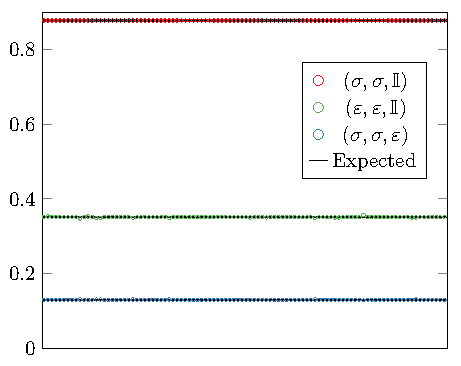
\includegraphics[width=\textwidth]{bootstrap_ising_3.pdf}
\end{minipage}
\vspace{0.75cm}

\begin{minipage}{0.5\linewidth}
\centering
\begin{tabular}{|c|c|}
\multicolumn{2}{c}{$c=-22/5$}\\
\hline 
  $(h_1, h_2, h_3)$ &  $D_{h_1 h_2 h_3}$ \\ 
 \hline
 $(\varphi, \varphi, \mathbb{I})$ &  $\phantom{-}1.51982706 \, (8.9\times 10^{-6})$      \\
 $(\varphi, \varphi, \varphi)$ &    $-6.84471259 \, (8.5\times 10^{-6})$     \\
 \hline
\end{tabular}
\end{minipage}
\begin{minipage}{0.5\linewidth}
 \centering
 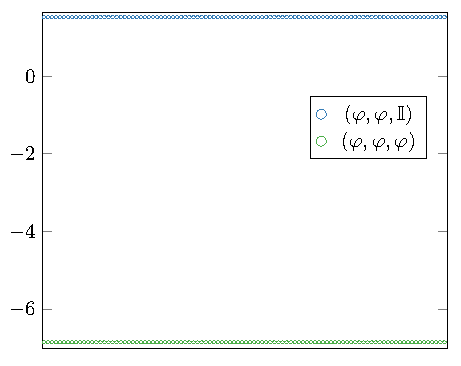
\includegraphics[width=\textwidth]{bootstrap_lee-yang_3.pdf}
\end{minipage}
\vspace{0.75cm}

\begin{minipage}{0.5\linewidth}
\centering
\begin{tabular}{|c|c|}
\multicolumn{2}{c}{$c=-3/5$}\\
\hline 
  $(h_1, h_2, h_3)$ &  $D_{h_1 h_2 h_3}$ \\ 
 \hline
 $(\sigma, \sigma, \mathbb{I})$ &            $\phantom{-}1.11011152\,(4.1\times10^{-4})$        \\
 $(\varepsilon, \varepsilon, \mathbb{I})$ &  $\phantom{-}0.65786020\,(1.0\times10^{-3})$        \\
 $(\psi, \psi, \mathbb{I})$   &              $\phantom{-}0.20732789\,(2.1\times10^{-2})$  \\
 $(\sigma, \sigma, \varepsilon)$ &           $-0.24661111\ (4.1\times 10^{-4})$\\
 $(\varepsilon, \varepsilon, \varepsilon)$ & $-2.33587779\, (2.2\times 10^{-3})$ \\
 $(\sigma, \varepsilon, \psi)$ &             $\phantom{-}0.09693064\,(1.1\times 10^{-2})$\\
 \hline
\end{tabular}
\end{minipage}
\begin{minipage}{0.5\linewidth}
 \centering 
 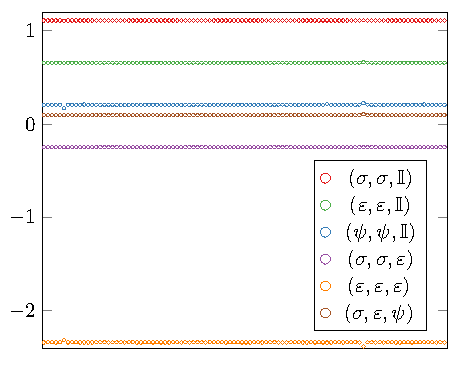
\includegraphics[width=\textwidth]{bootstrap_5-3_3.pdf}
\end{minipage}
\caption{\label{tab_bootstrap_results} Results of the numerical bootstrap for 
the Ising field theory (top), Lee-Yang model (center), and the Gaffnian theory (bottom) 
on a genus two surface ($N=3$). For each minimal model, the table on the left 
collects the mean value obtained for each structure constant after performing the bootstrap
with 100 different sets of random points $\{z_j\}$, fixing $\kappa=0.22$. The conformal block
expansion was truncated at level $\ell=6$. In the brackets we write the coefficient of variation.
In the figures on the right, we plot the values obtained for the structure constants
in each particular set of random points. These are the points employed to calculate the mean and 
standard deviation in the tables on the left. In the Ising theory case, the lines represent the values expected
for the structure constants: $D_{\sigma\sigma\mathbb{I}}\approx 0.877383$, 
$D_{\varepsilon\varepsilon\mathbb{I}}\approx 0.351166$, and $D_{\sigma\sigma\varepsilon}\approx 0.129983$. }
\end{table}


\section{Conclusions}
In this paper we solved numerically the conformal bootstrap to calculate genus two partition functions of rational CFTs, $\mathcal{C}$, with $c<1$. In particular, we focussed on CFTs defined on genus two Riemann surfaces with $\mathbb Z_3$ symmetry, whose partition function can be also rewritten as a twist field four-point function in the orbifold $\mathcal{C}^{\otimes N}/\mathbb Z_N$. Our results extend the approach to higher genus CFTs discussed in~\cite{Cardy, Collier}. In particular we provided a regularization scheme to remove from the combinatorial expansion of the conformal block null vector contributions for $c<1$. We also proposed an algorithm to systematically expand the genus $N-1$ conformal blocks into sphere conformal blocks of central charge $Nc$. The latter are more suitable to implement numerical calculations, since they can represented recursively through Zamolodchikov formula.
Our main results are the exact numerical determinations of the genus two partition functions for the Ising, the Lee-Yang and the Gaffian CFT. The Ising case shows perfect agreement with the free bosonic string calculation in~\cite{Calabrese}.

There are a couple of possibile future directions that are worth to be mentioned. First, it would be useful to investigate whether our formalism can be extended to arbitray values of the genus $g=N-1$. This task involves the determination of the descendent $N$-point function in Eq.~\eqref{N-point} for a rational CFT.  We expect the latter to be analytic in $g$  at least for a free compactified boson, thus allowing to recover the results for the entanglement entropy and negativity discussed in~\cite{Calabrese, Furukawa, Calabrese09, CalabreseNeg, Grava} from a different route.
Also it will be important to understand if a recursive formula for higher genus conformal blocks, such as that put forward in~\cite{Cho}, can be effectively implemented when $c<1$, due to the additional null vector resonances.

\appendix
\section{Transformation properties of Virasoro descendents}\label{app_ward}

Consider a CFT on the Riemann sphere parameterized by $z$. The Virasoro 
generators are defined by their action on the fields,
\begin{equation}
\label{vir_ln}
 L_{-n}(z)\phi^{M}_h(z)=\oint_{C_{z}}\frac{dz'}{2\pi i}(z'-z)^{n+1}~T(z')~\phi^{M}_h(z),
\end{equation}
where $C_{z}$ is a closed contour containing $z$ and $T(z)$ is the stress energy tensor. 
From the current-current OPE,
\begin{equation}
T(z) T(0)= \frac{c}{z^4}+ \frac{2}{z^2} T(0)+\frac{1}{z}\partial T (0)+\text{regular terms},
\end{equation} 
one obtains the  Virasoro algebra
\begin{equation}
 [L_n(0), L_{m}(0)]\phi^{M}_h(0) =\left[(n-m) L_{n+m}(0)+\frac{c}{12}n(n^2-1)\delta_{n+m, 0}\right]\phi^{M}_h(0).
\end{equation}

The Virasoro generators acting on a field inserted at $z=\infty$ are given by
\begin{equation}\label{L_infty}
 L_{-n}(z=\infty)=-\oint_{C_{\infty}}\frac{dz}{2\pi i}z^{n+1}T(z).
\end{equation}
Let us see how these operators transform under a conformal map
$t \mapsto z(t)$. By recalling the transformation of the stress energy tensor 
when we apply it,
\begin{equation}
T(z)\mapsto \left(\frac{d z}{d t}\right)^{-2} T(t)-\frac{c}{12}\left\{z(t),t\right\},
\end{equation}
where $\{z(t),t\}$ is the Schwarzian derivative, the Virasoro descendent in Eq.~\eqref{L_infty}
is then transformed into the linear combination of descendents acting on the point
$t_\infty$ in the $t$-surface whose image is $z(t_\infty)=\infty$
\begin{equation}\label{Virasoro_transf}
 \mathcal{L}_{-n}(t_\infty)=-\oint_{C_{t_\infty}}\frac{dt}{2\pi i}
 \left(\frac{dz}{dt}\right)^{-1}[z(t)]^{n+1}\left[T(t)-\frac{c}{12}\{z(t), t\}\right],
\end{equation}
where $C_{t_\infty}$ is a contour encircling the point $t_\infty$, and $T(t)$ can be 
expressed as
\begin{equation}
 T(t)=\sum_{m\in\mathbb{Z}}(t-t_\infty)^{-n-2}L_m(t=t_\infty).
\end{equation}


In subsection~\ref{sec:genus_one}, we have employed the conformal map
in Eq.~\eqref{g_one_covering_map} to compute the orbifold three-point function
of Eq.~\eqref{C_2_X} in the case $N=2$. For this particular map, 
we can write down the expansion of the Virasoro descendents in Eq.~\eqref{Virasoro_transf}
by applying the residue theorem; if $n\geq 1$ it reads
\begin{equation}\label{vir_g1_1}
 \mathcal{L}_{-n}(t_{\infty})=\sum_{m\geq -n} a_{nm} L_{m}(t=t_{\infty})+\frac{c}{32}(n-1), \quad t_{\infty}=\{0,\infty\},
\end{equation}
with
\begin{equation}\label{vir_g1_2}
 a_{nm}=\frac{1}{4^n}\left[2^{2n+1}-\binom{2n+1}{m+n+1}{}_2F_1(1, m-n, m+n+2, -1)\right].
\end{equation}

In the case $N=3$, studied in subsection~\ref{sec:genus_two}, the orbifold three-point function of Eq.~\eqref{C_3_X} is calculated by
applying the conformal map of Eq.~\eqref{g_two_covering_map}. The images $\mathcal{L}_{-n}(t_\infty)$ of the Virasoro descendents 
$L_{-n}(z=\infty)$ under this map can be also obtained by using Eq.~\eqref{Virasoro_transf}. We have, for $n\geq 1$,
\begin{equation}\label{vir_g2} 
 \mathcal{L}_{-n}(t_\infty)=\sum_{m\geq n}a_{nm}^{t_\infty}L_{m}(t=t_{\infty})+\frac{c}{27}(n-1),
 \quad t_\infty=\{0, 1, \infty\}
\end{equation}
where the coefficients $a_{nm}^{t_\infty}$ can be determined in closed form from the residue theorem, see also Eq.~(2.9) of Ref.~\cite{Collier}.

The three-point correlations on the sphere that appear in the expansion in Eq.~\eqref{genus_two_conf_block} of the $N=3$ orbifold 
conformal block can be computed recursively by employing the following Ward identities~\cite{Teschner},
\begin{multline}
\label{wardvir1}
 \langle L_{-n}\phi_{h_1}^{M_1}|\phi_{h_2}^{M_2}(1)|\phi_{h_3}^{M_3}\rangle=
 \langle \phi_{h_1}^{M_1}|\phi_{h_2}^{M_2}(1)|L_n \phi_{h_3}^{M_3}\rangle \\
 +\sum_{m= 1}^n \binom{n+1}{m+1}\langle \phi_{h_1}^{M_1}|L_m \phi_{h_2}^{M_2}(1)|\phi_{h_3}^{M_3}\rangle,
\end{multline}
\begin{multline}
\label{wardvir2}
 \langle \phi_{h_1}^{M_1}|L_{-n}\phi_{h_2}^{M_2}(1)|\phi_{h_3}^{M_3}\rangle=
 \sum_{m=0}^\infty\binom{n+m-2}{m}
 \left[\langle L_{m+n} \phi_{h_1}^{M_1}|\phi_{h_2}^{M_2}(1)|\phi_{h_3}^{M_3}\rangle \right.\\ +
 \left. (-1)^n\langle \phi_{h_1}^{M_1}|\phi_{h_2}^{M_2}(1)|L_{m-1} \phi_{h_3}^{M_3}\rangle\right],
\end{multline}
and
\begin{equation}
 \langle \phi_{h_1}|\phi_{h_2}(1)|L_{-n}\phi_{h_3}\rangle=
 \langle L_{-n}\phi_{h_3}|\phi_{h_2}(1)|\phi_{h_1}\rangle.
\end{equation}


\section{Orbifold Virasoro sub-algebra}\label{app_orbifold_algebra}

In each sheet of the orbifold theory $\mathcal{C}^{\otimes N}/\mathbb{Z}_N$, we 
can consider a copy $\boldsymbol{T}^{(j)}(z)$, $j=1,\dots, N$, of the stress-energy tensor of 
the seed theory $\mathcal{C}$. Then the stress-energy tensor of the 
orbifold theory $\boldsymbol{T}(z)$ is 
\begin{equation}\label{hatT}
 \boldsymbol{T}(z)=\sum_{j=1}^N \boldsymbol{T}^{(j)}(z).
\end{equation}
It generates transformations affecting all the sheets in the same way. 
Its Fourier modes,
\begin{equation}
 \boldsymbol{L}_n=\oint_{C_0}\frac{dz}{2\pi i} z^{n+1}\boldsymbol{T}(z),
\end{equation}
where $C_0$ is a contour encircling the point $z=0$, are symmetric 
under the exchange of sheets, 
\begin{equation}
 \boldsymbol{L}_n=\sum_{j=1}^N \boldsymbol{L}_n^{(j)}, \quad 
 \boldsymbol{L}_n^{(j)}=\mathbb{I}\otimes \overset{j}{\cdots} \otimes L_{n}\otimes \cdots \otimes \mathbb{I},
\end{equation}
and form a Virasoro algebra, 
\begin{equation}\label{symm_virasoro_alg}
 [\boldsymbol{L}_n, \boldsymbol{L}_{m}]=(n-m)\boldsymbol{L}_{n+m}+\frac{Nc}{12}n(n^2-1)\delta_{n+m, 0},
\end{equation}
with central charge $Nc$.

\section{Entanglement entropy and logarithmic negativity}\label{app_ent}

Let us consider a generic quantum system that can be divided into two 
spatial regions, which we call $A$ and $B$, such that the total Hilbert 
space factorizes as $\mathcal{H}=\mathcal{H}_A\otimes \mathcal{H}_B$.
We suppose that the system is in a pure state $|\Psi\rangle\in\mathcal{H}$. 
Hence the state of susbsytem $A$ is described by the reduced density matrix
\begin{equation}\label{red_density_matrix}
\rho_A=\Tr_{\mathcal{H}_B}|\Psi\rangle\langle\Psi|,
\end{equation}
with $\Tr_{\mathcal{H}_B}$ denoting the partial trace in the space $\mathcal{H}_B$. 
The entanglement between regions $A$ and $B$ can be analysed using the moments of the 
reduced density matrix, $\Tr\rho_A^N$. In particular, the entanglement entropy 
\begin{equation}
 S_A=-\Tr(\rho_A\log \rho_A)
\end{equation}
can be obtained from the R\'enyi entanglement entropies 
\begin{equation}
 S_A^{(N)}=\frac{1}{1-N}\log\Tr\rho_A^N
\end{equation}
by performing the replica trick
\begin{equation}
 S_A=\lim_{N\to 1^+}S_A^{(N)}=-\lim_{N\to1^+}\frac{\partial}{\partial N}\Tr\rho_A^N.
\end{equation}
If subsystem $A$ consists of two disjoint regions $A_1$ and $A_2$, 
such that and $\mathcal{H}_A=\mathcal{H}_{A_1}\otimes\mathcal{H}_{A_2}$,
then one can consider the partial transpose $\rho_A^{T_2}$ of $\rho_A$. 
If $\{|e_j^{(l)}\rangle\}$ denotes a basis of the space $\mathcal{H}_{A_l}$, 
then the matrix elements of $\rho_A^{T_2}$ are defined as 
\begin{equation}\label{partial_transpose}
\langle e_{j_1}^{(1)}e_{k_1}^{(2)}| \rho_A^{T_2} |e_{j_2}^{(1)}e_{k_2}^{(2)}\rangle=
\langle e_{j_1}^{(1)}e_{k_2}^{(2)}| \rho_A |e_{j_2}^{(1)}e_{k_1}^{(2)}\rangle.
\end{equation}
The moments $\Tr(\rho_A^{T_2})^N$ encode the entanglement between regions $A_1$ and $A_2$. 
A particular measure of the entanglement between these two regions is for instance the 
logarithmic negativity,
\begin{equation}
 \mathcal{E}=\log|\Tr_A^{T_2}|,
\end{equation}
which can also be calculated through the replica trick 
\begin{equation}
 \mathcal{E}=\lim_{n_{\rm e}\to 1^+}\log\Tr(\rho_A^{T_2})^{n_{\rm e}},
\end{equation}
by taking the analytic continuation of the moments $\Tr(\rho_A^{T_2})^N$
with even exponent $N=n_{\rm e}$.


\section{$N=3$ orbifold conformal blocks for the Ising model}\label{app_ising}

For the Ising field theory, the conformal block decomposition of 
Eq.~\eqref{conformal_block_decomposition_0} for the twist-field 
four-point function with $N=3$ takes the form,
\begin{equation}
 \langle \sigma_3(0)\bar{\sigma}_3(z, \bar{z})\sigma_3(1)\bar{\sigma}_3(\infty)\rangle=
 |\mathcal{G}_{\frac{1}{2},\mathbb{I}\mathbb{I}\mathbb{I}}^{(3)}(z)|^2+
 3D_{\sigma\sigma\mathbb{I}}|\mathcal{G}_{\frac{1}{2},\sigma\sigma\mathbb{I}}^{(3)}(z)|^2+
 3D_{\varepsilon\varepsilon\mathbb{I}}|\mathcal{G}_{\frac{1}{2},\varepsilon\varepsilon\mathbb{I}}^{(3)}(z)|^2+
 3D_{\sigma\sigma\varepsilon}|\mathcal{G}_{\frac{1}{2},\sigma\sigma\varepsilon}^{(3)}(z)|^2.
\end{equation}
The genus-three conformal blocks above have the following 
expansions in terms of Virasoro sphere conformal blocks up to level $L=6$,
\begin{equation}
 \mathcal{G}_{\frac{1}{2},\mathbb{I}\mathbb{I}\mathbb{I}}^{(3)}(z)\sim
 \mathcal{F}_{\frac{3}{2}, 0}(z) + 
 \frac{3211264}{10451673} \mathcal{F}_{\frac{3}{2}, 4}(z) + 
 \frac{2097152}{4782969} \mathcal{F}_{\frac{3}{2}, 5}(z) + 
 \frac{68719476736}{114891698349}\mathcal{F}_{\frac{3}{2}, 6}(z),
\end{equation}
\begin{multline}
 \mathcal{G}_{\frac{1}{2},\sigma\sigma\mathbb{I}}^{(3)}(z)\sim
 \mathcal{F}_{\frac{3}{2},\frac{1}{8}}(z) + 
 \frac{1}{27} \mathcal{F}_{\frac{3}{2}, \frac{9}{8}}(z) + 
 \frac{2209}{10206} \mathcal{F}_{\frac{3}{2}, \frac{17}{8}}(z) + 
 \frac{590597}{1456542} \mathcal{F}_{\frac{3}{2}, \frac{25}{8}}(z) + 
 \frac{61593283775}{143065334376}\mathcal{F}_{\frac{3}{2}, \frac{33}{8}}(z) \\ + 
 \frac{13237693484267}{23444417678328}\mathcal{F}_{\frac{3}{2}, \frac{41}{8}}(z) + 
 0.23567191378271496433 \mathcal{F}_{\frac{3}{2}, \frac{49}{8}}(z),
\end{multline}
\begin{multline}
 \mathcal{G}_{\frac{1}{2},\varepsilon\varepsilon\mathbb{I}}^{(3)}(z)\sim
 \mathcal{F}_{\frac{3}{2}, 1}(z)+ 
 \frac{8}{27} \mathcal{F}_{\frac{3}{2}, 2}(z)+ 
 \frac{128}{1701}\mathcal{F}_{\frac{3}{2}, 3}(z) + 
 \frac{2458624}{2027349}\mathcal{F}_{\frac{3}{2}, 4}(z) + 
 \frac{204636160}{749863251}\mathcal{F}_{\frac{3}{2}, 5}(z) \\+ 
 \frac{141295616}{3008487501}\mathcal{F}_{\frac{3}{2},6}(z) + 
 0.39631743847866107572\mathcal{F}_{\frac{3}{2}, 7}(z),
\end{multline}
and
\begin{multline}
 \mathcal{G}_{\frac{1}{2},\sigma\sigma\varepsilon}^{(3)}(z)\sim
 \mathcal{F}_{\frac{3}{2}, \frac{5}{8}}(z) + 
 \frac{49}{27}\mathcal{F}_{\frac{3}{2}, \frac{13}{8}}(z) + 
 \frac{637}{486}\mathcal{F}_{\frac{3}{2}, \frac{21}{8}}(z) + 
 \frac{176647}{485514}\mathcal{F}_{\frac{3}{2}, \frac{29}{8}}(z) + 
 \frac{6395744863}{16585210728}\mathcal{F}_{\frac{3}{2}, \frac{37}{8}}(z) \\ + 
 \frac{528656973059}{285256271160}\mathcal{F}_{\frac{3}{2}, \frac{45}{8}}(z) + 
 1.29430156184648710695\mathcal{F}_{\frac{3}{2}, \frac{53}{8}}(z).
\end{multline}

For the Ising model, the function $\mathcal{R}_N(z)$ that appears in Eqs.~\eqref{F_n_cc}
and $\eqref{G_n_cc}$ is of the form
\begin{equation}\label{R_n_ising}
\mathcal{R}_N^{\text{Ising}}(z)=\frac{1}{2^{N-1}|\chartheta{\boldsymbol{0}}{\boldsymbol{0}}(\Omega(z))|}
\sum_{\boldsymbol{\varepsilon},\boldsymbol{\delta}}
\left|\chartheta{\boldsymbol{\varepsilon}}{\boldsymbol{\delta}} (\Omega(z))\right|,\quad z\in\mathbb{C},
\end{equation}
where
$$\chartheta{\boldsymbol{\varepsilon}}{\boldsymbol{\delta}} (\Omega)=
\sum_{\boldsymbol{m}\in\mathbb{C}^{N-1}}
e^{i\pi({\bf m}+{\bf \varepsilon})^t
\cdot \Omega({\bf m}+{\bf \varepsilon})+2\pi i 
({\bf m}+\boldsymbol{\varepsilon})^t\cdot \boldsymbol{\delta}}.
$$
The caracteristics $\boldsymbol{\varepsilon},\boldsymbol{\delta}\in\mathbb{C}^{N-1}$
have as components $0$ or $1/2$, and $\Omega(z)$ is the symmetric $(N-1)\times (N-1)$
matrix 
\begin{equation}\label{period_matrix}
\Omega_{rs}(z)=\frac{2 i}{N}\sum_{k=1}^{N-1}\sin\left(\frac{\pi k}{N}\right)
\cos\left[\frac{2\pi k}{N}(r-s)\right]\beta_{k/N}(z),
\end{equation}
in which
$$\beta_{k/N}(z)=\frac{_2F_1(k/N, 1-k/N, 1; 1-z)}{_2F_1(k/N, 1-k/N, 1; z)}.$$

\acknowledgments
We thank Andrea Cappelli and Sylvain Ribault for discussions.





% The bibliography will probably be heavily edited during typesetting.
% We'll parse it and, using the arxiv number or the journal data, will
% query inspire, trying to verify the data (this will probalby spot
% eventual typos) and retrive the document DOI and eventual errata.
% We however suggest to always provide author, title and journal data:
% in short all the informations that clearly identify a document.

\begin{thebibliography}{99}

\bibitem{Dubrovin} B. A. Dubrovin, A. T. Fomenko, S. P. Novikov, \textit{Modern Geometry---Methods and Applications Part II. The Geometry and Topology of Manifolds}, Springer (1985).

\bibitem{Whittaker} E.T. Whittaker, G. N. Watson, \emph{A Course in Modern Analysis}, Cambridge University Press (1950).

\bibitem{Lunin} O. Lunin, S. D. Mathur, \emph{Correlation functions for $M(N)/S(N)$ orbifolds}, \href{https://doi.org/10.1007/s002200100431}{\emph{Commun. Math. Phys.} {\bf 219} (2001) 399-442}.

\bibitem{Dixon} L. Dixon, D. Friedan, E. Martinec, S. Shenker, \textit{The conformal field theory of orbifolds}, 
\href{https://doi.org/10.1016/0550-3213(87)90676-6}{\emph{Nucl. Phys. B} {\bf 282} (1987) 13-73}.

\bibitem{DiFrancesco} P. Di Francesco, P. Mathieu, D. Senechal, \textit{Conformal field theory}, Springer (1999)

\bibitem{Knizhnik} V. G. Knizhnik, \emph{Analytic fields on Riemannian surfaces. II}, 
\href{https://doi.org/10.1007/BF01225373}{\emph{Commun. Math. Phys.} {\bf 112}, 567-590 (1987)}.

\bibitem{CardyMod} J. Cardy, \emph{Operator content of two-dimensional conformally invariant theories}, 
\href{https://doi.org/10.1016/0550-3213(86)90552-3}{\emph{Nucl. Phys. B} {\bf 270} [FS16] (1986) 186-204}.

\bibitem{Cappelli} A. Cappelli, C. Itzykson, J.-B. Zuber, \emph{Modular invariant partition functions in two dimensions}, 
\href{https://doi.org/10.1016/0550-3213(87)90155-6}{\emph{Nucl. Phys.B} {\bf 280} [FS18], 445 (1987)}.

\bibitem{Cappelli2} A. Cappelli, C. Itzykson, J.-B. Zuber, \emph{The A-D-E classification of minimal and $A_1^{(1)}$ conformal invariant theories}, \href{https://doi.org/10.1007/BF01221394}{\emph{Commun. Math. Phys.} {\bf 113}, 1-26 (1987)}.

\bibitem{Cardy} J. Cardy, A. Maloney, H. Maxfield, \emph{A new handle on three-point coefficients: OPE asymptotics from genus
two modular invariance}, \href{https://doi.org/10.1007/JHEP10(2017)136}{\emph{JHEP} {\bf 10} (2017) 136}.

\bibitem{ZamolodchikovAT} Al. B. Zamolodchikov, \emph{Conformal scalar field on the hyperelliptic curve and critical Ashkin-Teller multipoint correlation functions}, \href{https://doi.org/10.1016/0550-3213(87)90350-6}{\emph{Nucl. Phys. B} {\bf 63} [FS19] (1987) 481-503}.

\bibitem{BPZ} A. Belavin, A. Polyakov, A. B. Zamolodchikov. \emph{Infinite conformal symmetry in two-dimensional quantum field theory},
\href{https://doi.org/10.1016/0550-3213(84)90052-X}{\emph{Nucl. Phys. B}, {\bf 241} (1984) 333-380}.

\bibitem{Friedan} D. Friedan, Z. Qiu, S. Shenker, \emph{Conformal Invariance, Unitarity, and Critical Exponents in Two Dimensions}, \href{https://doi.org/10.1103/PhysRevLett.52.1575}{\emph{Phys. Rev. Lett}. {\bf 52}, 1575 (1984)}.

\bibitem{Collier} M. Cho, S. Collier, X. Yin, \emph{Genus two modular bootstrap}, \href{https://doi.org/10.1007/JHEP04(2019)022}{\emph{JHEP} {\bf 04} (2019) 22}.

\bibitem{Ribault} S. Ribault, \emph{Conformal field theory on the plane}, \href{https://arxiv.org/abs/1406.4290}{\texttt{arXiv:1406.4290 [hep-th]}}.

\bibitem{Zamolodchikov2} Al.  B.  Zamolodchikov, \emph{Conformal  Symmetry  in  Two  Dimensions: An  Explicit  Recurrence Formula for the  Conformal Partial  Wave  Amplitude}, \href{https://doi.org/10.1007/BF01214585}{\emph{Commun. Math. Phys.} {\bf 96},  419-422  (1984)}.

\bibitem{SV} R. Santachiara, J. Viti, \emph{Local logarithmic correlators as limits of Coulomb gas integrals},
\href{https://doi.org/10.1016/j.nuclphysb.2014.02.022}{\emph{Nucl. Phys. B} {\bf 882} (2014) 229-262}.

\bibitem{Javerzat} N. Javerzat, R. Santachiara, O. Foda, \emph{Notes on the solutions of Zamolodchikov-type recursion relations in Virasoro minimal models}, \href{https://doi.org/10.1007/JHEP08(2018)183}{\emph{JHEP} {\bf 08} (2018) 183}.

\bibitem{Alkalaev} K. B. Alkalaev, V. A. Belavin, \emph{Conformal blocks of $\mathcal{W}_N$
minimal models and AGT correspondence}, \href{https://doi.org/10.1007/JHEP07(2014)024}{\emph{JHEP} {\bf 07} (2014) 024}.

\bibitem{SR} S. Ribault, R. Santachiara, \textit{Liouville theory with a central charge less than one}, 
\href{https://doi.org/10.1007/JHEP08(2015)109}{\emph{JHEP} {\bf 08} (2015) 109}.

\bibitem{Zamolodchikov} Al. B. Zamolodchikov, \emph{Conformal symmetry in two-dimensional space: Recursion representation of conformal
block}, \href{https://doi.org/10.1007/BF01022967}{\emph{Theor. Math. Phys.} {\bf 73}, 1088-1093  (1987)}.

\bibitem{Mussardo} G. Mussardo, \emph{Statistical Field Thoery: An Introduction to Exactly Solved Models in Statistical Physics}, Oxford University Press (2020).

\bibitem{Simon} S H. Simon, E. H. Rezayi, N. R. Cooper, I. Berdnikov, \emph{Construction of a paired wave function for spinless electrons at filling fraction $\nu=2/5$}, \href{https://doi.org/10.1103/PhysRevB.75.075317}{\emph{Phys. Rev. B} {\bf 75}, 075317 (2007)}.

\bibitem{Ardonne} E. Ardonne, J. Gukelberger, A. W. W. Ludwig, S. Trebst, M. Troyer, \emph{Microscopic models of interacting Yang-Lee anyons},
\href{https://doi.org/10.1088/1367-2630/13/4/045006}{\emph{New J. Phys.} {\bf 13} (2011) 045006}.

\bibitem{Calabrese} P. Calabrese, J. Cardy, E. Tonni, \emph{Entanglement entropy of two disjoint intervals in conformal field theory II}, \href{https://doi.org/10.1088/1742-5468/2011/01/P01021}{\emph{J. Stat. Mech} P01021 (2011)}.

\bibitem{Rajabpour} M. A. Rajabpour, F. Gliozzi, \emph{Entanglement entropy of two disjoint intervals from fusion algebra of twist fields},
\href{https://doi.org/10.1088/1742-5468/2012/02/P02016}{J. Stat. Mech. (2012) P02016}.

\bibitem{Ruggiero} P. Ruggiero, P. Calabrese, E. Tonni, \emph{Entanglement entropy of two disjoint intervals and the recursion formula
for conformal blocks}, \href{https://doi.org/10.1088/1742-5468/aae5a8}{\emph{J. Stat. Mech.} (2018) 113101}.

\bibitem{Furukawa}  S. Furukawa, V. Pasquier, J. Shiraishi, \emph{Mutual Information and Boson Radius in $c=1$ Critical Systems in One Dimension}, \href{https://doi.org/10.1103/PhysRevLett.102.170602}{\emph{Phys. Rev. Lett.} {\bf 102}, 170602 (2009)}.

\bibitem{Calabrese09} P. Calabrese, J. Cardy, E. Tonni, \emph{Entanglement entropy of two disjoint intervals in conformal field theory},
\href{https://doi.org/10.1088/1742-5468/2009/11/P11001}{J. Stat. Mech (2009) P11001}.

\bibitem{CalabreseNeg} P. Calabrese, J. Cardy, E. Tonni, \emph{Entanglement negativity in extended systems:  A field theoretical approach},
\href{https://doi.org/10.1088/1742-5468/2013/02/P02008}{J. Stat. Mech. (2013) P02008}.

\bibitem{Grava} T. Grava, A. P. Kels, E. Tonni, \emph{Entanglement of two disjoint intervals in CFT and the 2D Coulomb gas in a lattice},
\href{https://arxiv.org/abs/2104.06994}{\texttt{arXiv:2104.06994 [hep-th]}}.

\bibitem{Cho} M. Cho, S. Collier, X. Yin, \emph{Recursive representations of arbitrary Virasoro conformal blocks}, 
\href{https://doi.org/10.1007/JHEP04(2019)018}{\emph{JHEP} {\bf 04} (2019) 018}.

\bibitem{Teschner} J. Teschner, \emph{Liouville theory revisited}, \href{https://doi.org/10.1088/0264-9381/18/23/201}{\emph{Class. Quantum Grav.} {\bf 18} (2001) R153-R222}.

\bibitem{FS} D. Friedan, S. Shenker, \emph{The analytic geometry of two-dimensional conformal field theories}, \href{https://doi.org/10.1016/0550-3213(87)90418-4}{\emph{Nucl. Phys. B} {\bf 281} (1987) 509-545}.

\bibitem{Gaberdiel} M. R. Gaberdiel, C. A. Keller, R. Volpato, \emph{Genus two partition functions of chiral conformal field theories},
\href{https://dx.doi.org/10.4310/CNTP.2010.v4.n2.a2}{\emph{Commun. Num. Theor. Phys.} {\bf 4} (2010) 295-364}.

\bibitem{Headrick} M. Headrick, A. Maloney, E. Perlmutter, I. G. Zadeh, \emph{Renyi Entropies, the Analytic Bootstrap, and 3D Quantum Gravity at Higher Genus}, \href{https://doi.org/10.1007/JHEP07(2015)059}{\emph{JHEP} {\bf 07} (2015) 059}.

\bibitem{Keller} C. A. Keller, G. Mathys, I. G. Zadeh, \emph{Bootstrapping chiral CFTs at genus two},
\href{https://dx.doi.org/10.4310/ATMP.2018.v22.n6.a3}{\emph{Adv. Theor. Math. Phys.} {\bf 22} (2018) 1447-1487}

\bibitem{Dupic} T. Dupic, B. Estienne, Y. Ikhlef, \emph{Entanglement entropies of minimal models from null-vectors}, 
\href{https://scipost.org/10.21468/SciPostPhys.4.6.031}{\emph{SciPost Phys.} {\bf 4}, 031 (2018)}

\bibitem{Borisov} L. Borisov, M. B. Halpern, C. Schweigert, \emph{Systematic approach to cyclic orbifolds}, 
\href{https://doi.org/10.1142/S0217751X98000044}{\emph{Int. J. Mod. Phys. A} {\bf 13}, 125 (1998)}

\bibitem{Maldacena} J. Maldacena, D. Simmons-Duffin, A. Zhiboedov, \emph{Looking for a bulk point},
\href{ https://doi.org/10.1007/JHEP01(2017)013}{\emph{JHEP} {\bf 01} (2017) 013}

\bibitem{Rattazzi} R. Rattazzi, V. S. Rychkov, E. Tonni, A. Vichi, \emph{Bounding scalar operator dimensions in 4D CFT},
\href{https://doi.org/10.1088/1126-6708/2008/12/031}{\emph{JHEP} {\bf 12} (2008) 031}

\bibitem{Poland} D. Poland, S. Rychkov, A. Vichi, \emph{The Conformal Bootstrap: Theory, Numerical Techniques, and Applications},
\href{https://doi.org/10.1103/RevModPhys.91.015002}{\emph{Rev. Mod. Phys.} {\bf 91}, 015002 (2019)}

% Please avoid comments such as "For a review'', "For some examples",
% "and references therein" or move them in the text. In general,
% please leave only references in the bibliography and move all
% accessory text in footnotes.

% Also, please have only one work for each \bibitem.


\end{thebibliography}
\end{document}
